\chapter{Espacios Métricos}

\section{Preámbulo}

Las siguientes son notas de clase sobre el tema de Análisis Real, combinando recursos del curso de Cálculo Diferencial e Integral III del M. en C. Francisco Giovanni López Sánchez, y del curso de Análisis Matemático I del Dr. Fidel Casarrubias Segura, ambos impartidos en la Facultad de Ciencias de la UNAM, en el semestre 2024-1 y 2024-2 respectivamente. 

\section{Definición y Ejemplos}

\begin{definition}[Espacio Métrico] \label{def1}
    Sea $X$ un conjunto no vacío. Sea $d: X \times X \to \R \: \bigcup \: \{ 0 \}$ una función. Decimos que $d$ es una métrica o distancia en $X \Leftrightarrow d$ satisface las siguientes propiedades
    \begin{enumerate}[label=(\subscript{D}{{\arabic*}})]
        \item $\forall \: x,y \in X \Rightarrow d(x,y) \geqslant 0$ 
        \item $d(x,y) = 0 \Leftrightarrow x=y$
        \item $\forall \: x,y \in X \Rightarrow d(x,y) = d(y,x)$
        \item $\forall \: x,y,z \in X \Rightarrow d(x,z) \leqslant d(x,y) + d(y,z)$
    \end{enumerate}
   Un espacio métrico es una pareja ordenada $(X,d)$ donde $X$ es un conjunto no vacío y $d$ es una métrica en $X$.
\end{definition}

\begin{remark}
    $d(x,y)$ se lee como la distancia de $x$ a $y$
\end{remark}

\begin{eg}[Métrica Euclidiana]
    En ${\R}^{n}$, donde $n \in {\Z}^{+}$, la siguiente función $d: {\R}^{n} \times {\R}^{n} \to \R$ dada por:
    \begin{equation*}
        d(x,y) = \sqrt{\sum_{i=1}^{n} {({x}_{i}-{y}_{i})}^{2}}
    \end{equation*}
    donde $x=({x}_{1},...,{x}_{n})$ y  $y=({y}_{1},...,{y}_{n})$ es una métrica en ${\R}^{n} $
\end{eg}
\begin{explanation}
Por demostrar que la función anterior es una métrica en $\R^n$
    \begin{enumerate}[label=(\subscript{D}{{\arabic*}})]
        \item Por definición de raíz cuadrada de un número real, $d(x,y) \geqslant 0 \: \: \: \forall \: x,y \in {\R}^{n}$
        \item $\Longrightarrow$ Sea $x=({x}_{1},...,{x}_{n})$ y $y = ({y}_{1},...,{y}_{n}) \in {\R}^{n}$ P.D. $(D_2)$

        Supongamos que $d(x,y)=0$. Por definición de raíz cuadrada, notemos que $d(x,y)=0 \Leftrightarrow ({{x}_{i}-{y}_{i})}^{2} = 0$. Este termino es cero $\Leftrightarrow$ ambos elementos son el mismo vector en $\R^n$.

        $\Longleftarrow$ Supongamos que $x=y$. Al ser vectores en $\R^n$, $x=y \Leftrightarrow ({x}_{1}={y}_{1},...,{x}_{n}={y}_{n})$

        \begin{equation*}
            \Rightarrow d(x,y) = d(x,x)
        \end{equation*}
        \begin{equation*}
            \Rightarrow d(x,x) = \sqrt{\sum_{i=1}^{n} {({x}_{i}-{x}_{i})}^{2}} = \sqrt{\sum_{i=1}^{n} {0}^{2}} = 0
        \end{equation*}
        
        \item Sea $x=({x}_{1},...,{x}_{n})$ y $y = ({y}_{1},...,{y}_{n}) \in {\R}^{n}$ P.D. $(D_3)$

        Notemos que
        \begin{equation*}
        d(y,x) = \sqrt{\sum_{i=1}^{n} {({y}_{i}-{x}_{i})}^{2}} = \sqrt{\sum_{i=1}^{n} {{(-1)}^{2}({x}_{i}-{y}_{i})}^{2}} = \sqrt{\sum_{i=1}^{n} {({x}_{i}-{y}_{i})}^{2}} = d(x,y)
        \end{equation*}
        
        \item Sea $x=({x}_{1},...,{x}_{n})$, $y = ({y}_{1},...,{y}_{n})$ y $z = ({z}_{1},...,{z}_{n}) \in {\R}^{n}$ P.D. $(D_4)$        
    \end{enumerate}
\end{explanation}
\begin{aff}[Young Patito]
            $\forall \: a,b \in \R \Rightarrow ab \leqslant \frac{a^2+b^2}{2}$
        \end{aff}
        \begin{explanation}
            Sean cualesquiera $a,b \in \R$  

            Como $(a-b)^2 \geqslant 0 \Rightarrow$
            \begin{equation*}
                a^2-2ab+b^2 \geqslant 0
            \end{equation*}
            \begin{equation*}
                \Rightarrow 2ab \leqslant a^2+b^2 \Rightarrow \frac{a^2+b^2}{2} \geqslant ab
            \end{equation*}
        \end{explanation}
        \begin{aff}[Cauchy–Bunyakovsky–Schwarz]\label{aff1}
            $\forall \: a=({a}_{1},...,{a}_{n})$ y $b=({b}_{1},...,{b}_{n}) \in \R^n$
            \begin{equation*}
                \abs{\sum_{i=1}^{n} {a}_{i}{b}_{i}}  \leqslant \sqrt{\sum_{i=1}^{n} {{a}_{i}}^{2}} \sqrt{\sum_{i=1}^{n} {{b}_{i}}^{2}}
            \end{equation*}
        \end{aff}
        \begin{explanation}
            Sea $a=({a}_{1},...,{a}_{n})$ y $b=({b}_{1},...,{b}_{n}) \in \R^n$ elementos cualesquiera. Observe que para probar C-B-S es suficiente probar 
            \begin{equation}
                \sum_{i=1}^{n} \abs{{a}_{i}}\abs{{b}_{i}} \leqslant \sqrt{\sum_{i=1}^{n} {{a}_{i}}^{2}} \sqrt{\sum_{i=1}^{n} {{b}_{i}}^{2}} \label{eq1}
            \end{equation}
            Esto porque 
            \begin{equation*}
                \abs{\sum_{i=1}^{n} {a}_{i}{b}_{i}} \leqslant \sum_{i=1}^{n} \abs{{a}_{i}}\abs{{b}_{i}}
            \end{equation*}
            Para probar esto último, consideremos los siguientes dos casos.
            \begin{enumerate}[label=\alph*)]
                \item $a=\vec{0}$
                
                Si $a=\vec{0} \Rightarrow$ cada $a_i = 0$. De donde
                \begin{equation*}
                    \sum_{i=1}^{n} \abs{{a}_{i}}\abs{{b}_{i}} = 0\leqslant \sqrt{\sum_{i=1}^{n} {{a}_{i}}^{2}} \sqrt{\sum_{i=1}^{n} {{b}_{i}}^{2}}
                \end{equation*}
                \item $b=\vec{0}$
                
                Siguiendo un arguménto análogo al caso (1), s.t.q. 
                \begin{equation*}
                    \sum_{i=1}^{n} \abs{{a}_{i}}\abs{{b}_{i}} = 0\leqslant \sqrt{\sum_{i=1}^{n} {{a}_{i}}^{2}} \sqrt{\sum_{i=1}^{n} {{b}_{i}}^{2}}
                \end{equation*}

                \item $a \neq \vec{0}$ y $b \neq \vec{0}$

                Defina 
                \begin{align*}
                    \alpha = \sqrt{\sum_{i=1}^{n} {{a}_{i}}^{2}} & & \text{y} & & \beta = \sqrt{\sum_{i=1}^{n} {{b}_{i}}^{2}}
                \end{align*}
                Note que como $a \neq \vec{0}$ y $b \neq \vec{0} \Rightarrow \alpha > 0$ y $\beta >0$

                Observe que (\ref{eq1}) es equivalente a 
                \begin{equation}
                    \frac{\sum\limits_{i=1}^{n} \abs{{a}_{i}}\abs{{b}_{i}}}{\alpha \beta} \leqslant 1\label{eq2}
                \end{equation}

                Así, basta probar (\ref{eq2}). Para demostrar (\ref{eq2}), note que:
                \begin{equation*}
                    \frac{\sum\limits_{i=1}^{n} \abs{{a}_{i}}\abs{{b}_{i}}}{\alpha \beta} = \sum_{i=1}^{n} \frac{\abs{{a}_{i}}}{\alpha}\frac{\abs{{b}_{i}}}{\beta}
                \end{equation*}

                Aplicando la \Cref{aff1}, obtenemos que:
                \begin{equation*}
                    \sum_{i=1}^{n} \frac{\abs{{a}_{i}}}{\alpha}\frac{\abs{{b}_{i}}}{\beta} \leqslant \sum_{i=1}^{n} \frac{{\left(\frac{\abs{{a}_{i}}}{\alpha}\right)}^{2}+\left(\frac{\abs{{b}_{i}}}{{\beta}}\right)^{2}}{2}
                \end{equation*}
                \begin{equation*}
                    \frac{\frac{{\abs{{a}_{1}}}^{2}}{{\alpha}^{2}}+\frac{{\abs{{b}_{1}}}^{2}}{{\beta}^{2}}+...+\frac{{\abs{{a}_{n}}}^{2}}{{\alpha}^{2}}+\frac{{\abs{{b}_{n}}}^{2}}{{\beta}^{2}}}{2}
                \end{equation*}
                \begin{equation*}
                    \frac{\frac{{\abs{{a}_{1}}}^{2}+...+{\abs{{a}_{n}}}^{2}}{{\alpha}^{2}}+\frac{{\abs{{b}_{1}}}^{2}+...+{\abs{{b}_{n}}}^{2}}{{\beta}^{2}}}{2} = \frac{1+1}{2} = \frac{2}{2} = 1
                \end{equation*}
                Por lo tanto, (\ref{eq2}) es verdadero. 
            \end{enumerate}
        \end{explanation}
        \begin{aff}[$D_4$]
            $\forall \: x=({x}_{1},...,{x}_{n})$, $y=({y}_{1},...,{y}_{n})$ y $z=({z}_{1},...,{z}_{n}) \in \R^n$ s.t.q.
            \begin{equation*}
                d(x,z) \leqslant d(x,y) + d(y,z)
            \end{equation*}
        \end{aff}
        \begin{proofexplanation}
            Sean $x,y,z \in \R^n$ arbitrarios. P.D. ($D_4$). Observe que probar ($D_4$) es equivalente a probar 
            \begin{equation*}
                d(x,z)^2 \leqslant (d(x,y) + d(y,z))^2
            \end{equation*}
            Definamos $a_i = x_i-y_i$ y $b_i = y_i-z_i \: \forall \: i = 1,...,n$. Note que $\forall \: i = 1,...,n \Rightarrow x_i-z_i = a_i+b_i$.

            Tenemos lo siguiente
            \begin{equation*}
                 \sum_{i=1}^{n} (x_i-z_i)^2 =  \sum_{i=1}^{n} (a_i+b_i)^2 = \sum_{i=1}^{n} {a_i}^{2} + 2 \sum_{i=1}^{n} {a_i}{b_i} + \sum_{i=1}^{n} {b_i}^{2}
            \end{equation*}
            \begin{equation*}
                \leqslant \sum_{i=1}^{n} {a_i}^{2} + 2 \abs{\sum_{i=1}^{n} {a_i}{b_i}} + \sum_{i=1}^{n} {b_i}^{2} \leqslant \sum_{i=1}^{n} {a_i}^{2} + 2 \sqrt{\sum_{i=1}^{n} {a_i}^{2}}\sqrt{\sum_{i=1}^{n} {b_i}^{2}} + \sum_{i=1}^{n} {b_i}^{2}
            \end{equation*}
            \begin{equation*}
                {\left( \sqrt{\sum_{i=1}^{n} {a_i}^{2}} + \sqrt{\sum_{i=1}^{n} {b_i}^{2}}\right)}^{2} =  {\left( \sqrt{\sum_{i=1}^{n} {x_i-y_i}^{2}} + \sqrt{\sum_{i=1}^{n} {y_i-z_i}^{2}}\right)}^{2}
            \end{equation*}
            \begin{equation*}
                \Rightarrow \sum_{i=1}^{n} (x_i-z_i)^2 \leqslant {\left( \sqrt{\sum_{i=1}^{n} {x_i-y_i}^{2}} + \sqrt{\sum_{i=1}^{n} {y_i-z_i}^{2}}\right)}^{2} 
            \end{equation*}

            Es decir
            \begin{equation*}
                d(x,z)^2 \leqslant (d(x,y) + d(y,z))^2
            \end{equation*}

            Sacando la raíz cuadrado, s.t.q. ($D_4$) es verdadero.

            $\therefore d$ es una métrica en $\R^n$
        \end{proofexplanation}

\begin{eg}[Métrica Discreta]
    Sea $X$ un conjunto arbitrario no vacío. En $X \times X$ la siguiente función es una métrica en $X$
    \begin{equation*}
        d(x,y) = 
     \begin{cases}
              1 & \text{si } x \neq y,\\
              0 & \text{si } x = y
     \end{cases}
    \end{equation*}
\end{eg}

\begin{proofexplanation}    
    \begin{enumerate}[label=(\subscript{D}{{\arabic*}})]
    \item Sean cualesquiera $x,y \in X$. Tenemos los siguientes casos.
    \begin{enumerate}
        \item $x=y$

        En este caso, por definición de $d$
        \begin{equation*}
            d(x,y) = 0 \geqslant 0
        \end{equation*}
        
        Por propiedades de la igualdad, esto es verdadero.
        \item $x \neq y$

        En este caso, por definición de $d$

        \begin{equation*}
            d(x,y) = 1 \geqslant 0
        \end{equation*}
    \end{enumerate}
    \item Sean cualesquiera $x,y \in X$.

    $\Rightarrow$

    Si $d(x,y)=0 \Rightarrow x=y$, porque de lo contrario, por definición de $d$, $d(x,y)=1$ y en consecuencia $d(x,y)\neq0$

    $\Leftarrow$

    Por otro lado, si $x=y$, aplicando la definición de $d$, obtenemos que $d(x,y) = 0$

    \item Sean cualesquiera $x,y \in X$. Tenemos los siguientes casos.

    \begin{enumerate}
        \item $x=y$

        En este caso, como $x=y \Rightarrow y=x$, s.t.q.

        \begin{align*}
        d(x,y)=0 & & \text{y} & & d(y,x) =0
        \end{align*}

        $\Rightarrow d(x,y) = d(y,x)$

        \item $x\neq y$

        Primero, observemos que la implicación $y=x \Rightarrow x=y$ es equivalente a $x\neq y \Rightarrow y \neq x$. Consecuentemente, por definición de $d$

        \begin{align*}
        d(x,y)=1 & & \text{y} & & d(y,x) =1
        \end{align*}

        $\Rightarrow d(x,y) = d(y,x)$
    \end{enumerate}
    \item Sean cualesquiera $x,y,z \in X$. Para $x,z$ tenemos los siguientes casos.
    \begin{enumerate}
        \item $x=z$

        Debido a que la suma de numeros reales no negativos es no negativa, y por ($D_1$)
        \begin{align*}
        d(x,y) \geqslant 0 & & \text{y} & & d(y,x) \geqslant 0
        \end{align*}
        \begin{equation*}
            \Rightarrow d(x,z) = 0 \leqslant d(x,y) + d(y,z)
        \end{equation*}
        
        \item $x\neq z$

        Observe que, como $x=y$ y $y=z \Rightarrow x=z$, no puede ocurrir que
        \begin{align*}
        x=y & & \text{y} & & y=z
        \end{align*}

        Puesto que, por hipótesis, $x \neq z$
        \begin{align*}
        \Rightarrow x\neq y & & \text{o} & & y \neq z
        \end{align*}

        Si $x\neq y \Rightarrow d(x,y) = 1$. Luego
        \begin{equation*}
            d(x,z) = 1 = d(x,y) \leqslant d(x,y) + d(y,z)
        \end{equation*}

        Por otro lado, si  $y \neq z \Rightarrow d(x,z) = 1$. Luego
        \begin{equation*}
            d(y,z) = 1 = d(y,z) \leqslant d(x,y) + d(y,z)
        \end{equation*}

        Esto porque $d(x,y) \geqslant 0 $ por ($D_1$).

        
        

    \end{enumerate}
    \end{enumerate}
    $\therefore d$ es una métrica en $X$
\end{proofexplanation}

\begin{eg}
    Sean $X=(X,{d}_{x})$ y $X=(X,{d}_{y})$ espacios métricos consideramos el producto cartesiano
    
    \begin{equation*}
        X \times Y = \{ (x,y) \mid x \in X, y \in Y \}
    \end{equation*}

    Dados $({x}_{1},{y}_{1}), ({x}_{2},{y}_{2}) \in X \times Y$, definimos
    \begin{equation*}
        {d}_{p}[({x}_{1},{y}_{1}), ({x}_{2},{y}_{2})] = {[{d}_{x}{({x}_{1},{x}_{2})}^{p}+{d}_{y}{({y}_{1},{y}_{2})}^{p}]}^{\frac{1}{p}}
    \end{equation*}
    \begin{equation*}
        {d}_{\infty}[({x}_{1},{y}_{1}), ({x}_{2},{y}_{2})] = \max \{ {d}_{x}({x}_{1},{x}_{2})+{d}_{y}({y}_{1},{y}_{2}) \}
    \end{equation*}
\end{eg}

\begin{explanation}
    Supongamos que $p \in [0,\infty]$ es cualquier elemento. Tenemos los siguientes casos:
\end{explanation}

\begin{proofexplanation}
    \textcolor{ForestGreen!70!black}{\textbf{1) $p \in [1,\infty)$}} Sean $(x_1,y_1), (x_2,y_2), (x_3,y_3) \in X \times Y$ cualesquiera elementos.

    \begin{enumerate}[label=(\subscript{D}{{\arabic*}})]
    \item Notemos que, como ${d}_{x}$ y ${d}_{y}$ son métricas en $X$ y $Y$ respectivamente $\Rightarrow {d}_{x}{({x}_{1},{x}_{2})} \geqslant 0$ y ${d}_{y}{({y}_{1},{y}_{2})} \geqslant 0$. Esto implica $ {d}_{x}{({x}_{1},{x}_{2})}^{p} \geqslant 0$ y ${d}_{y}{({y}_{1},{y}_{2})}^{p} \geqslant 0$. De esto se sigue que:
    \begin{equation*}
         {d}_{p}[({x}_{1},{y}_{1}), ({x}_{2},{y}_{2})] = {[{d}_{x}{({x}_{1},{x}_{2})}^{p}+{d}_{y}{({y}_{1},{y}_{2})}^{p}]}^{\frac{1}{p}} \geqslant 0
    \end{equation*}
    \item $\Rightarrow$ 
    
    Supongamos que ${d}_{p}[({x}_{1},{y}_{1}), ({x}_{2},{y}_{2})] = 0$

    \begin{equation*}
        \Rightarrow {[{d}_{x}{({x}_{1},{x}_{2})}^{p}+{d}_{y}{({y}_{1},{y}_{2})}^{p}]}^{\frac{1}{p}} = 0
    \end{equation*}

    Con lo cual, s.t.q 

    \begin{equation*}
        {d}_{x}{({x}_{1},{x}_{2})}^{p}+{d}_{y}{({y}_{1},{y}_{2})}^{p} = 0
    \end{equation*}
    
    Como ${d}_{x}$ y ${d}_{y}$ son métricas $\Rightarrow {d}_{x}{({x}_{1},{x}_{2})} \geqslant 0$ y ${d}_{y}{({y}_{1},{y}_{2})} \geqslant 0$.

    Por ello, necesariamente que ${d}_{x}{({x}_{1},{x}_{2})}^{p}+{d}_{y}{({y}_{1},{y}_{2})}^{p} = 0 \Rightarrow$

        \begin{align*}
        {d}_{x}{({x}_{1},{x}_{2})} = 0 & & \text{y} & & {d}_{y}{({y}_{1},{y}_{2})} = 0
        \end{align*}

        Nuevamente usando que $d_x$ y $d_y$ son métricas s.t.q 
        
        \begin{align*}
        {d}_{x}{({x}_{1},{x}_{2})} = 0 \Rightarrow x_1 = x_2 & & \text{y} & & {d}_{y}{({y}_{1},{y}_{2})} = 0 \Rightarrow y_1 = y_2
        \end{align*}

        Es decir, $({x}_{1},{x}_{2}) = ({y}_{1},{y}_{2})$ 

        $\Leftarrow$

        Supongamos que $({x}_{1},{x}_{2}) = ({y}_{1},{y}_{2})$

        Como $d_x$ y $d_y$ son métricas en $X$ y $Y$ respectivamente s.t.q 

        \begin{align*}
        {d}_{x}{({x}_{1},{x}_{2})} = 0 & & \text{y} & & {d}_{y}{({y}_{1},{y}_{2})} = 0
        \end{align*}
        \begin{equation*}
            {[{d}_{x}{({x}_{1},{x}_{2})}^{p}+{d}_{y}{({y}_{1},{y}_{2})}^{p}]}^{\frac{1}{p}} = 0
        \end{equation*}

        Es decir, ${d}_{p}[({x}_{1},{y}_{1}), ({x}_{2},{y}_{2})]$

        \item Notemos que, como ${d}_{x}{({x}_{1},{x}_{2})} = {d}_{x}{({x}_{2},{x}_{1})}$  y ${d}_{y}{({y}_{1},{y}_{2})} = {d}_{y}{({y}_{2},{y}_{1})}$ s.t.q.

        \begin{equation*}
            {[{d}_{x}{({x}_{1},{x}_{2})}^{p}+{d}_{y}{({y}_{1},{y}_{2})}^{p}]}^{\frac{1}{p}} = {[{d}_{x}{({x}_{2},{x}_{1})}^{p}+{d}_{y}{({y}_{2},{y}_{1})}^{p}]}^{\frac{1}{p}}
        \end{equation*}
        \begin{equation*}
            \Rightarrow {d}_{p}[({x}_{1},{y}_{1}), ({x}_{2},{y}_{2})] = {d}_{p}[({x}_{2},{y}_{2}), ({x}_{1},{y}_{1})]
        \end{equation*}

        \item Refiérase a los apuntes de clase
    \end{enumerate}
\end{proofexplanation}

\begin{proofexplanation}
    \textcolor{ForestGreen!70!black}{\textbf{2) $p  = \infty$}}

    \smallskip
    
    Refiérase a los apuntes de clase

    \end{proofexplanation}

\begin{eg}
Sea $d$ una métrica en $\mathbb{R}^{n}$. Demuestra que la siguiente función es métrica en $\mathbb{R}^{n}$.

\begin{equation*}
    {d}_{m}(x,y)=\min(\{1,d(x,y)\})
\end{equation*}

\end{eg}
\begin{proofexplanation}
    

\begin{enumerate}[label=(\subscript{D}{{\arabic*}})]
\item  Sean $x,y \in \mathbb{R}^{n}$ P.D. ${d}_{m}(x,y) \geqslant 0$

Si ${d}(x,y)>1 \Rightarrow {d}_{m}(x,y)=1$. Si  ${d}(x,y)\leqslant 1 \Rightarrow {d}_{m}(x,y)=d(x,y)$. Tenemos los siguientes casos.

\begin{enumerate}
    
\item  ${d}(x,y) > 1 \Rightarrow {d}_{m}(x,y)=1 $

\begin{equation*}
    1 > 0 \Rightarrow {d}_{m}(x,y) \geqslant 0
\end{equation*}

\item ${d}(x,y) \leqslant 1 \Rightarrow {d}_{m}(x,y)={d}(x,y) $ Por definición,  $d(x,y) \geqslant 0$, $\Rightarrow {d}_{m}(x,y)\geqslant 0$

\end{enumerate}

\item Sean $x,y \in \mathbb{R}^{n}$ P.D. ${d}_{m}(x,y) = 0 \Leftrightarrow x=y$

 \begin{equation*}
     {d}_{m}(x,y) = 0 \Leftrightarrow \min(\{1,d(x,y)\}) = 0 \Leftrightarrow d(x,y) = 0 \Leftrightarrow x=y
 \end{equation*}

\item   Sean $x,y \in \mathbb{R}^{n}$ P.D. ${d}_{m}(x,y) ={d}_{m}(y,x) $

\begin{equation*}
     {d}_{m}(x,y) = \min(\{1,d(x,y)\}) = \min(\{1,d(y,x)\}) = {d}_{m}(y,x)
\end{equation*}

\item  Sean $x,y \in \mathbb{R}^{n}$ P.D. ${d}_{m}(x,z) \leqslant {d}_{m}(x,y) +{d}_{m}(y,z)$. Tenemos los siguientes casos.

\begin{enumerate}
    \item  Si ${d}(x,y) > 1 \Rightarrow {d}_{m}(x,y)=1 $ o ${d}(y,z) > 1 \Rightarrow {d}_{m}(y,z)=1 $

Notemos que, por definición, ${d}_{m}(x,z) \leqslant 1$

\begin{equation*}
    {d}_{m}(x,y) +{d}_{m}(y,z) \geqslant 1
\end{equation*}
\begin{equation*}
    {d}_{m}(x,z) \leqslant 1 \leqslant {d}_{m}(x,y) +{d}_{m}(y,z) \Rightarrow
\end{equation*}
\begin{equation*}
    {d}_{m}(x,z) \leqslant {d}_{m}(x,y) +{d}_{m}(y,z)
\end{equation*}


\item Si ${d}(x,y) < 1 \Rightarrow {d}_{m}(x,y)={d}(x,y) $ o ${d}(y,z) < 1 \Rightarrow {d}_{m}(y,z)={d}(y,z) $

\begin{equation*}
    {d}_{m}(x,y)+{d}_{m}(y,z)= {d}(x,y)+{d}(y,z) \geqslant {d}(x,z) \geqslant {d}_{m}(x,z) \Rightarrow
\end{equation*}
\begin{equation*}
    {d}_{m}(x,z) \leqslant {d}_{m}(x,y) +{d}_{m}(y,z)
\end{equation*}

\end{enumerate}
\end{enumerate}

$\therefore {d}_{m}(x,y)$ es una métrica en $\mathbb{R}^{n}$
\end{proofexplanation}


\begin{eg}
    

Sea $\rho$ una métrica en $\mathbb{R}^{n}$. Demuestra que la siguiente función es métrica en $\mathbb{R}^{n}$.

\begin{equation*}
    {\rho}_{1}(x,y)=\frac{\rho(x,y)}{1+\rho(x,y)}
\end{equation*}

\end{eg}

\begin{proofexplanation}
\begin{enumerate}[label=(\subscript{D}{{\arabic*}})]
\item  Sean $x,y \in \mathbb{R}^{n}$ P.D. ${\rho}_{1}(x,y) \geqslant 0$. 
        
Notemos que, ${\rho}(x,y) \geqslant 0$

\begin{equation*}
     \Rightarrow 1+{\rho}(x,y) \geqslant 0
    \Rightarrow \frac{{\rho}(x,y)}{1+{\rho}(x,y)} \geqslant 0    \Rightarrow {\rho}_{1}(x,y) \geqslant 0
\end{equation*}

\item  Sean $x,y \in \mathbb{R}^{n}$ P.D. ${\rho}_{1}(x,y)=0 \Leftrightarrow x=y$

\begin{equation*}
    {\rho}_{1}(x,y)=0 \Leftrightarrow \frac{{\rho}(x,y)}{1+{\rho}(x,y)} = 0
\end{equation*}

    Si $b \neq 0$ $\Rightarrow \frac{a}{b}=0 \Leftrightarrow a = 0$

\begin{equation*}
    \frac{{\rho}(x,y)}{1+{\rho}(x,y)} = 0 \Leftrightarrow {\rho}(x,y) = 0 \Leftrightarrow x = y
\end{equation*}

\item  Sean $x,y \in \mathbb{R}^{n}$ P.D. ${\rho}_{1}(x,y)={\rho}_{1}(y,x)$

\begin{equation*}
    {\rho}_{1}(x,y)= \frac{{\rho}(x,y)}{1+{\rho}(x,y)}=\frac{{\rho}(y,x)}{1+{\rho}(y,x)}= {\rho}_{1}(y,x)
\end{equation*}

\item  Sean $x,y \in \mathbb{R}^{n}$ P.D. ${\rho}_{1}(x,z) \leqslant {\rho}_{1}(x,y) +{\rho}_{1}(y,z)$

\begin{equation*}
    {\rho}_{1}(x,z) =\frac{{\rho}(x,z)}{1+{\rho}(x,z)} = \frac{1+{\rho}(x,z)-1}{1+{\rho}(x,z)}
\end{equation*}

\begin{equation*}
    = \frac{1+{\rho}(x,z)}{1+{\rho}(x,z)}-\frac{1}{1+{\rho}(x,z)}=1-\frac{1}{1+{\rho}(x,z)}
\end{equation*}

\begin{equation*}
    \leqslant 1-\frac{1}{1+{\rho}(x,y)+{\rho}(y,z)}=\frac{1+{\rho}(x,y)+{\rho}(y,z)-1}{1+{\rho}(x,y)+{\rho}(y,z)}
\end{equation*}

\begin{equation*}
    =\frac{{\rho}(x,y)+{\rho}(y,z)}{1+{\rho}(x,y)+{\rho}(y,z)}=\frac{{\rho}(x,y)}{1+{\rho}(x,y)+{\rho}(y,z)}+\frac{{\rho}(y,z)}{1+{\rho}(x,y)+{\rho}(y,z)}
\end{equation*}

\begin{equation*}
    \leqslant \frac{{\rho}(x,y)}{1+{\rho}(x,y)}+\frac{{\rho}(y,z)}{1+{\rho}(y,z)}={\rho}_{1}(x,y)+{\rho}_{1}(y,z) 
\end{equation*}

\begin{equation*}
    \Rightarrow {\rho}_{1}(x,z) \leqslant {\rho}_{1}(x,y)+{\rho}_{1}(y,z)
\end{equation*}
\end{enumerate}

$\therefore {\rho}_{1}(x,y)$ es una métrica en $\mathbb{R}^{n}$.
\end{proofexplanation}



\section{Espacios Normados}


\begin{definition}[Norma]
    Sea $V$ un espacio vectorial sobre $\R$. Una norma en $V$ es una función $\norm{\cdot} : V \to \R$ que tiene las siguientes propiedades
    \begin{enumerate}[label=(\subscript{N}{{\arabic*}})]
    \item $\forall \: x \in V \Rightarrow \norm{x} \geqslant 0$
    \item $\norm{x} = 0 \Leftrightarrow x = \vec{0}$, donde $\vec{0}$ es el neutro aditivo de $V$
    \item $\forall \: x \in V$ y $\forall \: \lambda \in \R \Rightarrow \norm{\lambda x} = \abs{\lambda} \norm{x}$
    \item $\forall \: x,y \in V \Rightarrow \norm{x+y} \leqslant \norm{x} + \norm{y}$
    \end{enumerate}
\end{definition}

\begin{theorem}\label{theom1}
    Si $\norm{\cdot}$ es una norma en un espacio vectorial real $X \Rightarrow$ la función $f : X \times X \to \R$ definida por

    \begin{equation*}
        d(x,y) = \norm{x+(-y)}
    \end{equation*}

    Con $x,y \in X$ es una métrica en $X \backepsilon$

    \begin{enumerate}[label=\alph*)]
    \item $\forall \: x, y \in X$ y $\forall \: \lambda \in \R$ $\Rightarrow d(\lambda x, \lambda y) = \abs{\lambda} \cdot d(x,y)$
    \item  $\forall \: x, y, z \in X$ $\Rightarrow d(x+z, y+z) = d(x,y)$
    \end{enumerate}
\end{theorem}

\begin{proof}
    \begin{enumerate}[label=(\subscript{D}{{\arabic*}})]
    \item Por ($N_1$) si $x,y \in X$ son elementos arbitrarios $\Rightarrow d(x,y) = \norm{x+(-y)} \geqslant 0$ ya que $x+(-y) \in X$
    \item Sean $x,y \in X$ elementos arbitrarios. Por ($N_2$)

    \begin{equation*}
     \norm{x+(-y)} = 0 \Leftrightarrow x+(-y) = \vec{0}
    \end{equation*}

    Luego $d(x,y) = 0 \Leftrightarrow x=y$

    \item  Sean $x,y \in X$ elementos arbitrarios. Notemos que 

    \begin{equation*}
         d(x,y) = \norm{x+(-y)} = \norm{(-1)(-x)+(-1)(y)}
    \end{equation*}
    \begin{equation*}
         = \norm{(-1)(y-x)} = \abs{1} \norm{y-x} = \norm{y-x} = d(y,x)
    \end{equation*}

    \item Sean $x,y,z \in X$ elementos arbitrarios.

    \begin{equation*}
        d(x,z) = \norm{x+(-z)} = \norm{(x+\vec{0})+(-z)}
    \end{equation*}
    \begin{equation*}
        = \norm{(x+((-y)+y))+(-z)} = \norm{(x-y)+(y-z)}
    \end{equation*}
    \begin{equation*}
        \leqslant \norm{x-y} + \norm{y-z}
    \end{equation*}
    
    \item Sean $x,y \in X$ arbitrarios.

    \begin{equation*}
        d(\lambda x, \lambda y ) = \norm{\lambda x + -(\lambda)y} = \norm{\lambda(x-y)} = \abs{\lambda} \norm{x-y} = \abs{\lambda} \cdot d(x,y)
    \end{equation*}
    
    \item Sean $x,y,z \in X$ elementos arbitrarios.

    \begin{equation*}
        \Rightarrow d(x+z,y+z) = \norm{(x+z)-(y+z)} = \norm{(x+z)+(-1)(y+z)}
    \end{equation*}
    \begin{equation*}
        = \norm{(x+z)+(-1)y+(-1)z} = \norm{x-y} = d(x,y)
    \end{equation*}
    \end{enumerate}

    $\therefore$ el \Cref{theom1} se cumple.
\end{proof}

\begin{theorem} \label{theom2}
    $\forall \: p \in [1,\infty)$ y con $n \in {\Z}^{+}$ la función ${\norm{\cdot}}_{p} : \R^n \to \R$ definida por:

    \begin{equation*}
        {\norm{x}}_{p} = {\left( \sum_{i=1}^{n} {\abs{{x}_{i}}}^{p}\right)}^{\frac{1}{p}}
    \end{equation*}

    \noindent donde $x=(x_1,...,x_n)$ es una norma en $\R^n$ llamada norma $p$. La métrica que indúce es la métrica

    \begin{equation*}
        {d}_{p}(x,y) = {\norm{x+(-y)}}_{p} = {\left( \sum_{i=1}^{n} {\abs{{x}_{i}-{y}_{i}}}^{p}\right)}^{\frac{1}{p}}
    \end{equation*}
\end{theorem}

\begin{proof}
    \begin{enumerate}[label=(\subscript{D}{{\arabic*}})]
    \item Sea $x=(x_1,...,x_n) \in \R^n$ arbitrario. Tenemos los siguientes casos.
    \begin{enumerate}
        \item Si $x=\vec{0} \Rightarrow \abs{{x}_{i}} = 0 \: \forall \: i=1,...,n$

        Luego ${\abs{{x}_{i}}}^{p} = {0}^{p} = 0 \: \forall \: i=1,...,n$ 

        \begin{equation*}
            \Rightarrow  {\norm{x}}_{p} = {\left( \sum_{i=1}^{n} {\abs{{x}_{i}}}^{p}\right)}^{\frac{1}{p}} = {0}^{\frac{1}{p}}=0 
        \end{equation*}
        \item  Si $x \neq \vec{0} \Rightarrow x_{i_0} \neq 0$ para algún $i_0 \in \{ 1,...,n \}$

        Consecuentemente 

        \begin{equation*}
            \sum_{i=1}^{n} {\abs{{x}_{i}}}^{p} \geqslant {\abs{ x_{i_0}}}^{p} > 0
        \end{equation*}
        \begin{equation*}
            \Rightarrow  {\norm{x}}_{p} = {\left( \sum_{i=1}^{n} {\abs{{x}_{i}}}^{p}\right)}^{\frac{1}{p}} > 0 
        \end{equation*}
    \end{enumerate}
    \item Se sigue de la demostración del caso $a)$ de ($N_1$)
    \item Sean $x \in \R^n$ y $\lambda \in \R$ arbitrarios. Tenemos los siguientes casos.
    \begin{enumerate}
        \item Si $\lambda = 0 \Rightarrow \lambda x = \vec{0}$ y $\abs{\lambda}=0$. Luego

        \begin{equation*}
              {\norm{\lambda x}}_{p} =   {\norm{\vec{0}}}_{p} = 0 = 0 \cdot {\norm{x}}_{p} = \lambda {\norm{x}}_{p} 
        \end{equation*}

        \item Si $x = \vec{0} \Rightarrow \lambda x = \vec{0}$ y ${\norm{x}}_{p}=0$. Consecuentemente

        \begin{equation*}
              {\norm{\lambda x}}_{p} =   {\norm{\vec{0}}}_{p} = 0 = \abs{\lambda} \cdot 0 = \lambda {\norm{x}}_{p} 
        \end{equation*}

        \item Finalmente si $\lambda \neq 0 $ y $ x \neq \vec{0} \Rightarrow \lambda x \neq 0$

        Así, $\exists \: i_0 \in \{ 1,...,n \} \backepsilon \abs{\norm{ \lambda {{x}_{i}}_{0}}} < 0$

        Luego 

         \begin{equation*}
            \sum_{i=1}^{n} {\abs{\lambda {x}_{i}}}^{p} \geqslant {\abs{\lambda x_{i_0}}}^{p} > 0
        \end{equation*}
        \begin{equation*}
            \Rightarrow  {\norm{\lambda x}}_{p} = {\left( \sum_{i=1}^{n} {\abs{\lambda {x}_{i}}}^{p}\right)}^{\frac{1}{p}} = \exp ({\ln {\left( \sum\limits_{i=1}^{n} {\abs{\lambda {x}_{i}}}^{p}\right)}^{\frac{1}{p}}})
        \end{equation*}
        \begin{equation*}
            = \exp({ {\frac{1}{p}} \ln  {\left( \sum\limits_{i=1}^{n} {\abs{\lambda {x}_{i}}}^{p}\right)}}) = \exp( {\frac{1}{p}} {\ln {\left( \sum\limits_{i=1}^{n} {\abs{\lambda}}^{p} {\abs{{x}_{i}}}^{p} \right)}})
        \end{equation*}
        \begin{equation*}
            = \exp( {\frac{1}{p}} {\ln {\left( {\abs{\lambda}}^{p} \cdot \sum\limits_{i=1}^{n}  {\abs{{x}_{i}}}^{p} \right)}}) = \exp( {\frac{1}{p}} {\ln {\left( {\abs{\lambda}}^{p} \right)}} + {\frac{1}{p}} {\ln {\left( \sum\limits_{i=1}^{n}  {\abs{{x}_{i}}}^{p} \right)}})
        \end{equation*}
        \begin{equation*}
            \exp( {\frac{1}{p}} {\ln {\left[ {\abs{\lambda}}^{p} \right]}}) \cdot \exp( {\frac{1}{p}} {\ln {\left( \sum\limits_{i=1}^{n}  {\abs{{x}_{i}}}^{p} \right)}}) = \exp({\ln {\left[ \abs{\lambda} \right]}}) \cdot \exp( \ln {\left( \sum_{i=1}^{n} {\abs{{x}_{i}}}^{p}\right)}^{\frac{1}{p}} )
        \end{equation*}
        \begin{equation*}
            \abs{\lambda} \cdot {\left( \sum_{i=1}^{n} {\abs{{x}_{i}}}^{p}\right)}^{\frac{1}{p}} = \abs{\lambda} {\norm{x}}_{p}
        \end{equation*}
    \end{enumerate}
    \item Para probar la desigualdad triangular, debemos antes probar algunos lemas.
    \end{enumerate}
\end{proof}

\begin{lemma}[Desigualdad de Young] \label{lema1}
    Sean $p,q \in [1,\infty)$ elementos cualesquiera $\backepsilon \frac{1}{p}+\frac{1}{q} = 1$

    \begin{equation*}
        \Rightarrow ab \leqslant \frac{a^p}{p}+ \frac{b^q}{q} \: \: \: \: \: \: \: \: \forall \: a,b \in \R \:  \: \: \: \: \: \: \: \text{con } \:  a,b \geqslant 0
    \end{equation*}
\end{lemma}

\begin{proof}
    Sean $a,b \in \R$ con $a,b \geqslant 0$. Sin perder generalidad podemos suponer que $a > 0$ y $b > 0$. Tenemos los siguientes casos.

    \begin{enumerate}
        \item $a^p < b^q$

        Primero notemos que el número real 

        \begin{equation*}
            \frac{a^p}{p}+ \frac{b^q}{q} \in [a^p,b^q]
        \end{equation*}

        Ya que
        \begin{equation*}
            \frac{a^p}{p}+ \frac{b^q}{q} = a^p(1-t_0)+{b}^{q}{t}_{0}
        \end{equation*}

        Donde $t_0 = \frac{1}{q} \in [0,1]$

        Por otro lado, la ecuación de la línea recta en $\R^2$ que une a los puntos ($a^p,\ln(a^p)$), ($b^q,\ln(b^q)$) es 

        \begin{equation*}
            \frac{\ln(b^q)-\ln(a^p)}{b^q-a^p} \Rightarrow f(x) = \ln(a^p)+ \frac{\ln(b^q)-\ln(a^p)}{b^q-a^p} (x-a^p)
        \end{equation*}

        Debido a que la segunda derivada de $\ln = - \frac{1}{x^2} < 0 $ la función $\ln : (0,\infty) \to \R$ es cóncava en $(0,\infty)$, lo que significa, geométricamente, que la gráfica de $\ln$ está por encima de la función $f$.

        \begin{equation*}
            \implies \frac{a^p}{p}+ \frac{b^q}{q} \in [a^p,b^q] \implies f\left( \frac{a^p}{p}+ \frac{b^q}{q} \right) \leqslant \ln( \frac{a^p}{p}+ \frac{b^q}{q})
        \end{equation*}

        Pero

        \begin{equation*}
            f\left( \frac{a^p}{p}+ \frac{b^q}{q} \right) = \ln(a^p)+ \frac{\ln(b^q)-\ln(a^p)}{b^q-a^p} \left( \frac{a^p}{p}+ \frac{b^q}{q}-a^p \right)
        \end{equation*}
        \begin{equation*}
             = \ln(a^p)+ \frac{\ln(b^q)-\ln(a^p)}{b^q-a^p} \left( a^p  \left( \frac{1}{p}-1 \right)+ \frac{b^q}{q}-\right)
        \end{equation*}
        \begin{equation*}
             = \ln(a^p)+ \frac{\ln(b^q)-\ln(a^p)}{b^q-a^p} \left( a^p  \left( -\frac{1}{q} \right)+ \frac{b^q}{q}\right)
        \end{equation*}
        \begin{equation*}
             = \ln(a^p)+ \frac{\ln(b^q)-\ln(a^p)}{b^q-a^p} \left( \frac{1}{q} (b^q-a^p) \right)
        \end{equation*}
        \begin{equation*}
             = \ln(a^p) + \left( \frac{\ln(b^q)-\ln(a^p)}{q} \right) = \frac{\ln(a^p)}{q} + \frac{\ln(a^p)}{p}+ \frac{\ln(b^q)}{q}- \frac{\ln(a^p)}{q}
        \end{equation*}
        \begin{equation*}
              \frac{\ln(a^p)}{p}+ \frac{\ln(b^q)}{q} \leqslant \ln( \frac{a^p}{p}+ \frac{b^q}{q}) = \ln(ab) \leqslant \ln( \frac{a^p}{p}+ \frac{b^q}{q})
        \end{equation*}
        \begin{equation*}
            \Rightarrow ab \leqslant \frac{a^p}{p}+ \frac{b^q}{q}
        \end{equation*}

        Geométricamente, lo podemos ver de esta forma

    \begin{center}
    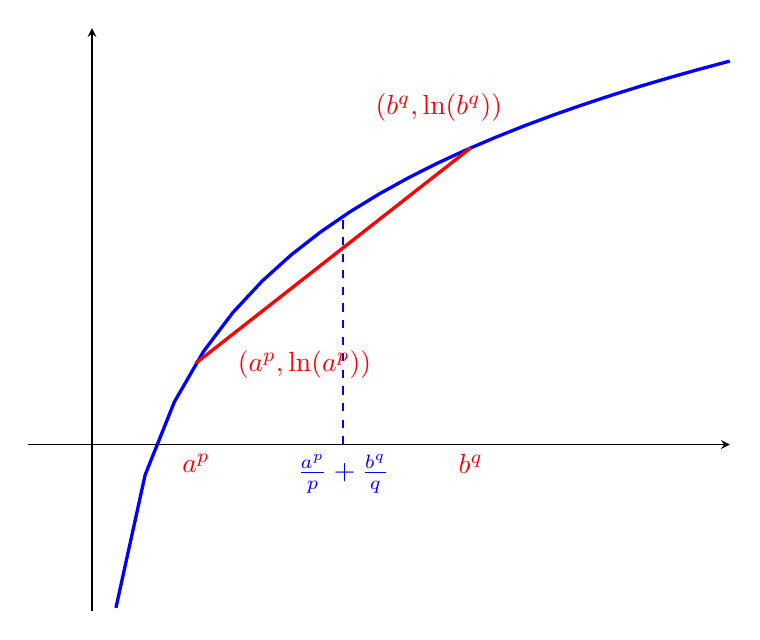
\begin{tikzpicture}
    \begin{axis}[
    scale = 1.3,
    xmin = -1, xmax = 10,
    ymin = -1, ymax = 2.5,
    axis x line=center,
    axis y line=center,
    xtick = {0}, ytick = \empty,
    clip = false,
    ]

    \addplot[color = blue, very thick, domain=-1:10] {ln(x)};
    \addplot[color = red, very thick, domain=1.631:5.938] {0.3*x};

    \addplot[color = blue, dashed, thick] coordinates { (3.938,0) (3.938, 1.373) };


    \node [above, red] at (axis cs: 5.438, 1.881) {$(b^q, \ln (b^q))$};
    \node [above, red] at (axis cs: 3.331, 0.339) {$(a^p, \ln (a^p))$};
    \node [below, red] at (axis cs: 1.631, 0) {$a^p$};
    \node [below, red] at (axis cs: 5.938, 0) {$b^q$};
    \node [below, blue] at (axis cs: 3.938, 0) {$\frac{a^p}{p}+ \frac{b^q}{q}$};

    
    \end{axis}
    \end{tikzpicture}
    \end{center}

        \item $b^q < a^p$

        Observe que 

        \begin{equation*}
            \frac{a^p}{p}+ \frac{b^q}{q} =  \frac{a^p}{p} + b^q \left( 1- \frac{1}{p} \right) \in [b^q,a^p]
        \end{equation*}

        Así que,

        \begin{equation*}
            f\left( \frac{a^p}{p}+ \frac{b^q}{q} \right) \leqslant \ln( \frac{a^p}{p}+ \frac{b^q}{q})
        \end{equation*}

        Por tanto, análogamente al caso anterior

        \begin{equation*}
            ab \leqslant \frac{a^p}{p}+ \frac{b^q}{q}
        \end{equation*}

        \item $a^p=b^q$

        Note que

        \begin{equation*}
            ab = {(a^p)}^{\frac{1}{p}}b = {(b^q)}^{\frac{1}{p}}b = {(b^q)}^{\frac{1}{p}}{(b^q)}^{\frac{1}{q}} = {(b^q)}^{\frac{1}{p}+\frac{1}{q}} 
        \end{equation*}
        \begin{equation*}
            =b^q = b^q \left(\frac{1}{p}+\frac{1}{q} \right) =   \frac{b^q}{p}+ \frac{b^q}{q}=  \frac{a^p}{p}+ \frac{b^q}{q}
        \end{equation*}
    \end{enumerate}

    $\therefore$ el \Cref{lema1} es verdadero.
\end{proof}

\begin{lemma}[Desigualdad de Hölder] \label{lema2}
    $\forall \: x,y \in \R^n $ s.t.q.

    \begin{equation*}
        \sum_{i=1}^{n} \abs{{x}_{i}{y}_{i}} \leqslant {\left( \sum_{i=1}^{n} {\abs{{x}_{i}}}^{p}\right)}^{\frac{1}{p}} {\left( \sum_{i=1}^{n} {\abs{{y}_{i}}}^{q}\right)}^{\frac{1}{q}}
    \end{equation*}

    donde $p,q \in [1,\infty)$, $\frac{1}{p}+\frac{1}{q} = 1$, $x=(x_1,...,x_n)$ y $y=(y_1,...,y_n)$
\end{lemma}

\begin{proof}
    Sean $x=(x_1,...,x_n)$ y $y=(y_1,...,y_n) \in \R^n$ cualesquiera elementos. Tenemos los siguientes casos.
    \begin{enumerate}
        \item $x= \vec{0}$

        Como $x= \vec{0} \Rightarrow x_i = 0 \: \forall \: i = 1,...,n$

        \begin{equation*}
        \sum_{i=1}^{n} \abs{{x}_{i}} \abs{{y}_{i}} = 0 \leqslant {\left( \sum_{i=1}^{n} {\abs{{x}_{i}}}^{p}\right)}^{\frac{1}{p}} {\left( \sum_{i=1}^{n} {\abs{{y}_{i}}}^{q}\right)}^{\frac{1}{q}}
    \end{equation*}

        \item $y= \vec{0}$
        
        Como $y= \vec{0} \Rightarrow y_i = 0 \: \forall \: i = 1,...,n$

        \begin{equation*}
        \sum_{i=1}^{n} \abs{{x}_{i}} \abs{{y}_{i}} = 0 \leqslant {\left( \sum_{i=1}^{n} {\abs{{x}_{i}}}^{p}\right)}^{\frac{1}{p}} {\left( \sum_{i=1}^{n} {\abs{{y}_{i}}}^{q}\right)}^{\frac{1}{q}}
    \end{equation*}

        \item  $x \neq \vec{0} \neq y$

        Como $x \neq \vec{0} \neq y$, definamos $\alpha = {\left( \sum\limits_{i=1}^{n} {\abs{{x}_{i}}}^{p}\right)}^{\frac{1}{p}} > 0$ y  $\beta = {\left( \sum\limits_{i=1}^{n} {\abs{{y}_{i}}}^{q}\right)}^{\frac{1}{q}} > 0$

        Definamos ahora a $a_i = \frac{\abs{x_i}}{\alpha}$ y $b_i = \frac{\abs{y_i}}{\beta}$. Por el \Cref{lema1} s.t.q.

        \begin{equation*}
        {a}_{i}{b}_{i} \leqslant \frac{{{a}_{i}}^{p}}{p} + \frac{{{a}_{i}}^{q}}{q} \: \: \: \: \: \: \: \: \: \: \: \: \forall \: i = 1,...,n
        \end{equation*}

        Es decir

        \begin{equation*}
           \frac{\abs{x_i}}{\alpha} \frac{\abs{y_i}}{\beta} \leqslant \frac{1}{p} \cdot\frac{{\abs{x_i}}^{p}}{\alpha^p} +  \frac{1}{q} \cdot\frac{{\abs{y_i}}^{q}}{\beta^q} \: \: \: \: \: \: \: \: \: \: \: \: \forall \: i = 1,...,n
        \end{equation*}
        
        \begin{equation*}
            \Rightarrow \sum_{i_1}^{n}\frac{\abs{x_i}}{\alpha} \frac{\abs{y_i}}{\beta} \leqslant \sum_{i_1}^{n} \left( \frac{1}{p} \cdot\frac{{\abs{x_i}}^{p}}{\alpha^p} +  \frac{1}{q} \cdot\frac{{\abs{y_i}}^{q}}{\beta^q} \right)
        \end{equation*}

        Consecuentemente
        \begin{equation*}
            \frac{ \sum\limits_{i=1}^{n} \abs{{x}_{i}} \abs{{y}_{i}}}{\alpha \beta} \leqslant \frac{1}{p} \cdot \frac{1}{\alpha^p} \sum\limits_{i=1}^{n} {\abs{{x}_{i}}}^{p} + \frac{1}{q} \cdot \frac{1}{\beta^q} \sum\limits_{i=1}^{n} {\abs{{y}_{i}}}^{q} = 1
        \end{equation*}
        
        \begin{equation*}
            \frac{ \sum\limits_{i=1}^{n} \abs{{x}_{i}} \abs{{y}_{i}}}{\alpha \beta} \leqslant 1 \Rightarrow \sum\limits_{i=1}^{n} \abs{{x}_{i}} \abs{{y}_{i}} \leqslant \alpha \beta
        \end{equation*}
    \end{enumerate}

    $\therefore$ el \Cref{lema2} es verdadero
\end{proof}

\begin{lemma}[Desigualdad de Minkowski]
    \begin{equation*}
        \forall \: x = (x_1,...,x_n), y = (y_1,...,y_n) \in \R^n \Rightarrow {\norm{x+y}}_{p} \leqslant {\norm{x}}_{p} + {\norm{y}}_{p}
    \end{equation*}
\end{lemma}

\begin{proof}
    Sean $x,y \in \R^n$ arbitrarios. Tenemos los siguientes casos.
    \begin{enumerate}
        \item $x= \vec{0}$

        Si $x=0 \Rightarrow x+y = y \Rightarrow {\norm{x}}_{p}  = 0$. Así que

        \begin{equation*}
            {\norm{x+y}}_{p} = {\norm{y}}_{p} = 0 + {\norm{y}}_{p} = {\norm{x}}_{p} + {\norm{y}}_{p}
        \end{equation*}

        \item $x \neq \vec{0}$

        Definamos a $\zeta = ({(\abs{{x}_{i}}+\abs{{y}_{i}})}^{p-1},...,{(\abs{{x}_{n}}+\abs{{y}_{n}})}^{p-1})$

        Aplicando el \Cref{lema2} a los vectores $ x = (x_1,...,x_n)$, a $\zeta$ y a $q=\frac{p}{p-1}$ s.t.q.

        \begin{equation*}
            \sum\limits_{i=1}^{n} \abs{{x}_{i}} {\left( \abs{{x}_{i}}+\abs{{y}_{i}} \right)}^{p-1} \leqslant {\left( \sum\limits_{i=1}^{n} {\abs{{x}_{i}}}^{p}\right)}^{\frac{1}{p}} {\left( \sum\limits_{i=1}^{n} {\left( {\left( \abs{{x}_{i}}+\abs{{y}_{i}} \right)}^{p-1}\right)}^{q} \right)}^{\frac{1}{q}}
        \end{equation*}

        De igual manera, aplicando el \Cref{lema2} a los vectores $ y = (y_1,...,y_n)$, y a $\zeta$ s.t.q.

        \begin{equation*}
            \sum\limits_{i=1}^{n} \abs{{y}_{i}} {\left( \abs{{x}_{i}}+\abs{{y}_{i}} \right)}^{p-1} \leqslant {\left( \sum\limits_{i=1}^{n} {\abs{{y}_{i}}}^{p}\right)}^{\frac{1}{p}} {\left( \sum\limits_{i=1}^{n} {\left( {\left( \abs{{x}_{i}}+\abs{{y}_{i}} \right)}^{p-1}\right)}^{q} \right)}^{\frac{1}{q}}
        \end{equation*}

        Note ahora que 

        \begin{equation*}
            \xi = {\left( \sum\limits_{i=1}^{n} \left( {\left( \abs{{x}_{i}}+\abs{{y}_{i}} \right)}^{q ({p-1})}\right)\right)}^{\frac{1}{q}} > 0 
        \end{equation*}

        Así, s.t.q.

        \begin{equation*}
            \sum\limits_{i=1}^{n} {\left( \abs{x_i}+\abs{y_i} \right)}^{p} = \sum\limits_{i=1}^{n} {\left( \abs{x_i}+\abs{y_i} \right)}{\left( \abs{{x}_{i}}+\abs{{y}_{i}} \right)}^{p-1}
        \end{equation*}
        \begin{equation*}
            =  \sum\limits_{i=1}^{n} \abs{{x}_{i}} {\left( \abs{{x}_{i}}+\abs{{y}_{i}} \right)}^{p-1} +  \sum\limits_{i=1}^{n} \abs{{y}_{i}} {\left( \abs{{x}_{i}}+\abs{{y}_{i}} \right)}^{p-1}
        \end{equation*}
        \begin{equation*}
            \leqslant \xi \cdot \left( {\left( \sum\limits_{i=1}^{n} {\abs{{x}_{i}}}^{p}\right)}^{\frac{1}{p}} + {\left( \sum\limits_{i=1}^{n} {\abs{{y}_{i}}}^{p}\right)}^{\frac{1}{p}}\right) = \xi \cdot ( {\norm{x}}_{p} + {\norm{y}}_{p})
        \end{equation*}

        Pero
        \begin{equation*}
            \frac{ \sum\limits_{i=1}^{n} {\left( \abs{x_i}+\abs{y_i} \right)}^{p}}{\xi} = \frac{\sum\limits_{i=1}^{n} {\left( \abs{x_i}+\abs{y_i} \right)}^{p}}{{\left( \sum\limits_{i=1}^{n} \left( {\left( \abs{{x}_{i}}+\abs{{y}_{i}} \right)}^{p}\right)\right)}^{\frac{1}{q}}} 
        \end{equation*}

        \begin{equation*}
            = {\left( \sum\limits_{i=1}^{n} \left( {\left( \abs{{x}_{i}}+\abs{{y}_{i}} \right)}^{p}\right)\right)}^{1-\frac{1}{q}} =  {\left( \sum\limits_{i=1}^{n} \left( {\left( \abs{{x}_{i}}+\abs{{y}_{i}} \right)}^{p}\right)\right)}^{\frac{1}{p}} \leqslant {\norm{x}}_{p} + {\norm{y}}_{p}
        \end{equation*}

        Finalmente

        \begin{equation*}
            {\norm{x + y}}_{p} = {\left( \sum\limits_{i=1}^{n} \left( {\left( \abs{{x}_{i}+{y}_{i}} \right)}^{p}\right)\right)}^{\frac{1}{p}} \leqslant {\left( \sum\limits_{i=1}^{n} \left( {\left( \abs{{x}_{i}}+\abs{{y}_{i}} \right)}^{p}\right)\right)}^{\frac{1}{p}} \leqslant {\norm{x}}_{p} + {\norm{y}}_{p}
        \end{equation*}
    \end{enumerate}

    $\therefore {\norm{\cdot}}_{p}$ es una norma y se cumple el \Cref{theom2}
\end{proof}

\begin{theorem} \label{theom113}
    
 Veamos que  ${\norm{x}}_{\infty} = \max \{ \abs{{x}_{i}} \mid i = 1,...,n\}$ donde $x=(x_1,...,x_n) \in \R^n$ es una norma en $\R^n$

 \end{theorem}

 \begin{lemma} \label{lematarea}
    Probaremos que, en general, $\forall \: \varepsilon > 0 $ y $y_1,...,y_n \in \R^n$ s.t.q. $\max \{ \varepsilon \cdot y_i \mid i = 1,...,n\} = \varepsilon \cdot \max \{  y_i \mid i = 1,...,n\}$ 
\end{lemma}

\begin{proof}
    Supongamos que $\varepsilon \cdot y_j = \max \{ \varepsilon \cdot y_i \mid i = 1,...,n\}$ para algún índice $j \in \{ 1,...,n \} \Rightarrow \: \forall \: i = 1,...,n $ s.t.q.

    \begin{equation*}
        y_i \leqslant \varepsilon \cdot y_i \leqslant \varepsilon \cdot y_j
    \end{equation*}

    Como $\varepsilon > 0 \Rightarrow y_i \leqslant y_j \: \forall \:   i = 1,...,n$ , es decir que

    \begin{equation*}
        y_j = \max \{ y_i \mid i = 1,...,n\}
    \end{equation*}

    Así que, como $ y_i \leqslant y_j \leqslant \varepsilon \cdot y_i \leqslant \varepsilon \cdot y_j$ , s.t.q.

    \begin{equation*}
        \varepsilon \cdot \max \{ y_i \mid i = 1,...,n\} \leqslant \max \{ \varepsilon \cdot y_i \mid i = 1,...,n\}
    \end{equation*}

    Por otra parte, como $y_j = \max \{ y_i \mid i = 1,...,n\} \Rightarrow \: \forall \: i = 1,...,n $ s.t.q.
    
    \begin{equation*}
         \varepsilon \cdot y_i \leqslant \varepsilon \cdot y_j
    \end{equation*}

    Como $\varepsilon > 0 \Rightarrow$

    \begin{equation*}
        \max \{ \varepsilon \cdot y_i \mid i = 1,...,n\} \leqslant \varepsilon \cdot y_j 
    \end{equation*}
    \begin{equation*}
        \max \{ \varepsilon \cdot y_i \mid i = 1,...,n\} \leqslant \varepsilon \cdot \max \{ y_i \mid i = 1,...,n\} 
    \end{equation*}
    \begin{equation*}
        \Rightarrow max \{ \varepsilon \cdot y_i \mid i = 1,...,n\} = \varepsilon \cdot \max \{ y_i \mid i = 1,...,n\} 
    \end{equation*}
\end{proof}

\begin{proof}

Podemos ahora demostrar el \Cref{theom113}

\begin{enumerate}[label=(\subscript{N}{{\arabic*}})]
\item $\forall \: (x_1,...,x_n) \in \R^n$ arbitrario s.t.q. $\abs{{x}_{i}} \geqslant 0 \: \forall \: i = 1,...,n$

\begin{equation*}
    \Rightarrow  \max \{ \abs{{x}_{i}} \mid i = 1,...,n\} ={\norm{x}}_{\infty} \geqslant 0
\end{equation*}

\item 

\begin{equation*}
    {\norm{x}}_{\infty} = 0 = \max \{ \abs{{x}_{i}} \mid i = 1,...,n\} \Leftrightarrow \abs{{x}_{i}} = 0 \: \forall \: i = 1,...,n \Leftrightarrow {x}_{i} = (0,...,0)
\end{equation*}

\item Sea $(x_1,...,x_n) \in \R^n$ y $\lambda \in \R$ arbitrarios

\begin{equation*}
    \Rightarrow {\norm{\lambda x}}_{\infty}  = \max \{ \abs{{\lambda x}_{i}} \mid i = 1,...,n\} = \max \{ \abs{\lambda } \abs{{\lambda x}_{i}} \mid i = 1,...,n\}
\end{equation*}

Para $\lambda \in \R$ tenemos los siguientes casos

\begin{enumerate}
    \item $\lambda = 0$

    En este caso $\lambda \cdot x = \vec{0}$ y por ($N_2$) s.t.q.

    \begin{equation*}
        {\norm{\lambda x}}_{\infty} = 0 = 0 \cdot {\norm{ x}}_{\infty}
    \end{equation*}

    \item $\lambda \neq 0 \Rightarrow \abs{\lambda} > 0$

    Por el \Cref{lematarea} anterior s.t.q.

    \begin{equation*}
        \max \{ \abs{\lambda } \abs{{\lambda x}_{i}} \mid i = 1,...,n\} = \abs{\lambda } \max \{  \abs{{\lambda x}_{i}} \mid i = 1,...,n\} = \abs{\lambda } {\norm{ x}}_{\infty}
    \end{equation*}
    
\end{enumerate}

\item Sean $x=(x_1,...,x_n)$ y $y=(y_1,...,y_n) \in \R^n$ arbitrarios. Por definición de ${\norm{ \cdot}}_{\infty}$ s.t.q.

\begin{equation*}
    {\norm{ x+y}}_{\infty} = \max \{ \abs{{x}_{i}+{y}_{i}} \mid i = 1,...,n\}
\end{equation*}

Supongamos que $\abs{x_j + y_j} = \max \{ \abs{{x}_{i}+{y}_{i}} \mid i = 1,...,n\}$

Como $\abs{x_j + y_j} \leqslant \abs{x_j} + \abs{y_j}$

\begin{equation*}
    \max \{ \abs{{x}_{i}+{y}_{i}} \mid i = 1,...,n\} \leqslant \abs{x_j} + \abs{y_j}
\end{equation*}
\begin{align*}
        \abs{x_j} \leqslant \max \{ \abs{{x}_{i}} \mid i = 1,...,n\} & & \text{y} & & \abs{y_j} \leqslant \max \{ \abs{{y}_{i}} \mid i = 1,...,n\}
\end{align*}

Por lo cual, por transitividad de $\leqslant$

\begin{equation*}
    \max \{ \abs{{x}_{i}+{y}_{i}} \mid i = 1,...,n\} \leqslant \max \{ \abs{{x}_{i}} \mid i = 1,...,n\} + \max \{ \abs{{y}_{i}} \mid i = 1,...,n\} 
\end{equation*}
\begin{equation*}
    \Rightarrow {\norm{ x+y}}_{\infty} \leqslant  {\norm{x}}_{\infty} +  {\norm{y}}_{\infty}
\end{equation*}
\end{enumerate}    

$\therefore {\norm{x}}_{\infty} = \max \{ \abs{{x}_{i}} \mid i = 1,...,n\}$ es una norma en $\R^n$
\end{proof}

\section{Espacios Con Producto Interior}

\begin{definition}[Espacios con producto interior]
    Recordemos que un espacio con producto interior es un espacio vectorial real $V$, en el cual se define una función $\langle \: , \: \rangle : V \times V \to \R$ llamada producto interior de $V$, que tiene las siguientes propiedades
        \begin{enumerate}[label=(\subscript{P}{{\arabic*}})]
        \item $\forall \: x,y \in V \Rightarrow \langle x,y \rangle = \langle y,x \rangle$
        \item $\forall \: x,y,z \in V \Rightarrow \langle x+z,y\rangle = \langle x,y \rangle+\langle z,y\rangle$
        \item  $\forall \: x,y \in V $ y $ \forall \: \lambda \in \R \Rightarrow \langle \lambda x,y \rangle = \lambda \langle x,y \rangle$
        \item $\forall \: x \in V  \Rightarrow \langle x,x \rangle \geqslant 0$
        \item $\forall \: x \in V  \Rightarrow \langle x,x \rangle = 0 \iff x = \vec{0}$
        \end{enumerate}
    De manera formal, un espacio con producto interior es una pareja ($V, \langle \: , \: \rangle$) donde $V$ es un espacio vectorial sobre $\R$ y  $\langle \: , \: \rangle$ es un producto interior en $V$.
\end{definition}

\begin{theorem}[Desigualdad de Cauchy - Schwarz] \label{theom3}
    Sea ($V, \langle \: , \: \rangle$) un espacio con producto interior, $ \implies  \forall \: x,y \in V$ s.t.q.

    \begin{equation*}
        \abs{\langle x,y \rangle} \leqslant \sqrt{\langle x,x \rangle} \cdot \sqrt{\langle y,y \rangle}
    \end{equation*}
\end{theorem}

\begin{proof}
    Sean $x,y \in V$ Para $y$ tomamos los siguientes casos

    \begin{enumerate}
        \item $y=\vec{0}$

        \begin{equation*}
            \Rightarrow \langle x,y \rangle = \langle y,x \rangle = \langle 0 \cdot \vec{0} \rangle = 0 \langle y,z \rangle = \vec{0}
        \end{equation*}
        \begin{equation*}
            \Rightarrow \abs{\langle x,y \rangle} = 0 \implies \abs{\langle x,y \rangle} = 0 \leqslant \sqrt{\langle x,x \rangle} \cdot \sqrt{\langle y,y \rangle} = \sqrt{\langle x,x \rangle} \cdot \sqrt{0} = 0
        \end{equation*}

        En este caso, se cumple la desigualdad.
        \item $y \neq \vec{0}$

        Resolvamos para $\lambda$ la siguiente ecuación 

        \begin{equation*}
            \langle x - \lambda y , \lambda y \rangle = 0
        \end{equation*}
        
        Note que 

        \begin{equation*}
            \langle x - \lambda y , \lambda y \rangle = 0 \iff \langle x , \lambda y \rangle - \langle \lambda y , \lambda y \rangle = 0
        \end{equation*}
        \begin{equation*}
            \Leftrightarrow \lambda \langle x,y \rangle - \lambda^2 \langle y,y \rangle = 0 \iff \lambda [ \langle x,y \rangle - \lambda \langle y ,y \rangle ] = 0
        \end{equation*}
        \begin{align*}
            \iff \lambda = 0& & \text{o} & & \langle x,y \rangle - \lambda \langle y ,y \rangle = 0
        \end{align*}

        Debido a que $\lambda \neq 0$ s.t.q

        $\lambda_0 = \frac{\langle x,y \rangle}{\langle y,y \rangle}$ es una solución no cero de lo anterior.

        Observe que la función $f : \R \to \R$ dada por 

        \begin{equation*}
            f(\lambda) = \langle x - \lambda y , x - \lambda y \rangle \geqslant 0
        \end{equation*}

        Sustituyendo a $\lambda_0$ en $f(\lambda) $ s.t.q. $f(\lambda_0) \geqslant 0 $

        Note ahora que
        \begin{equation*}
            0 \leqslant f(\lambda_0) = \langle x - \lambda_0 y , x - \lambda_0 y \rangle = \langle x , x \rangle + \langle x , - \lambda_0 y \rangle  + \langle - \lambda_0 y , x \rangle + \langle  - \lambda_0 y , - \lambda_0 y \rangle 
        \end{equation*}
        \begin{equation*}
            = \langle x , x \rangle -2 \lambda_0 \langle x , y \rangle +{\lambda}_{0}^{2} \langle y , y \rangle
            = \langle x , x \rangle -2 \frac{\langle x,y \rangle}{\langle y,y \rangle} \langle x , y \rangle +\frac{{\langle x,y \rangle}^{2}}{{\langle y,y \rangle}^{2}} \langle y , y \rangle 
        \end{equation*}
        \begin{equation*}
            = \langle x , x \rangle -2 \frac{{\langle x,y \rangle}^{2}}{\langle y,y \rangle} +\frac{{\langle x,y \rangle}^{2}}{\langle y,y \rangle} = \langle x , x \rangle - \frac{{\langle x,y \rangle}^{2}}{\langle y,y \rangle} 
        \end{equation*}
        \begin{equation*}
            \Rightarrow \frac{{\langle x,y \rangle}^{2}}{\langle y,y \rangle}  \leqslant \langle x , x \rangle \Rightarrow {\langle x,y \rangle}^{2} \leqslant \langle y,y \rangle \langle x , x \rangle 
        \end{equation*}
        \begin{equation*}
        \Rightarrow \abs{\langle x,y \rangle} \leqslant \sqrt{\langle x,x \rangle} \cdot \sqrt{\langle y,y \rangle}
    \end{equation*}
        
    \end{enumerate}

    $\therefore$ el \Cref{theom3} es cierto.
\end{proof}

\begin{theorem}[Desigualdad de Minkowski] \label{theom4}
    Sea ($V, \langle \: , \: \rangle$) un espacio con producto interior, $ \implies  \forall \: x,y \in V$ s.t.q.

    \begin{equation*}
        \sqrt{\langle x + y, x + y \rangle} \leqslant \sqrt{\langle x,x \rangle} + \sqrt{\langle y,y \rangle}
    \end{equation*}
\end{theorem}

\begin{proof}
    Sean $x, y \in V$ cualesquiera elementos. Note que

    \begin{equation*}
         \sqrt{\langle x + y, x + y \rangle} \leqslant \sqrt{\langle x,x \rangle} + \sqrt{\langle y,y \rangle} \Leftrightarrow \langle x + y, x + y \rangle \leqslant {(\sqrt{\langle x,x \rangle} + \sqrt{\langle y,y \rangle})}^{2}
    \end{equation*}
    \begin{equation*}
        \Leftrightarrow \langle x , x \rangle + 2 \langle x ,y \rangle + \langle y , y \rangle \leqslant \langle x , x \rangle + 2 \sqrt{\langle x,x \rangle} \cdot \sqrt{\langle y,y \rangle} + \langle y , y \rangle 
    \end{equation*}
    \begin{equation*}
        \langle x,y \rangle \leqslant \sqrt{\langle x,x \rangle} \cdot \sqrt{\langle y,y \rangle}
    \end{equation*}

    $\implies$ para probar \Cref{theom4} basta probar $\langle x,y \rangle \leqslant \sqrt{\langle x,x \rangle} \cdot \sqrt{\langle y,y \rangle}$

    Notemos que

    \begin{equation*}
        \langle x,y \rangle \leqslant \abs{\langle x,y \rangle}
    \end{equation*}

    Por el \Cref{theom3} s.t.q.

    \begin{equation*}
        \abs{\langle x,y \rangle} \leqslant \sqrt{\langle x,x \rangle} \cdot \sqrt{\langle y,y \rangle} \Rightarrow \langle x,y \rangle \leqslant \sqrt{\langle x,x \rangle} \cdot \sqrt{\langle y,y \rangle}
    \end{equation*}
\end{proof}

\begin{definition} \label{def14}
    Sea ($V, \langle \: , \: \rangle$) un espacio con producto interior. Definimos a la norma de $x \in V$ como el número $\in \R \backepsilon$

    \begin{equation*}
        \norm{x} := \sqrt{\langle x,x \rangle}
    \end{equation*}

    Note que $\norm{\cdot} : V \to \R$ es una función.
\end{definition}

\begin{theorem}
     Sea ($V, \langle \: , \: \rangle$) es un espacio vectorial real con producto interior $\Rightarrow$ la norma definida en la \Cref{def14} es una norma en $V$.
    
\end{theorem}

\begin{proof}
    \begin{enumerate}[label=(\subscript{N}{{\arabic*}})]
    \item Si $x \in V$ es un elemento arbitrario $\Rightarrow \langle x, x \rangle \geqslant 0$. Así que $\norm{x} = \sqrt{\langle x,x \rangle} \geqslant 0$
    \item Debido a que $\forall \: x \in V \Rightarrow \langle x, x \rangle = 0 \iff x = 0$, podemos concluir que $\forall \: x \in V \Rightarrow \norm{x} = 0 \iff x = 0$ puesto que 
    \begin{equation*}
        \sqrt{\langle x,x \rangle} = 0 \iff \langle x,x \rangle = 0 \implies \norm{x} = 0 \iff x = 0
    \end{equation*}
    \item Supongamos que $x \in V$ y $\lambda \in \R$ arbitrarios $\implies$ usando propiedades de $\langle \: , \: \rangle$ s.t.q.
    \begin{equation*}
        \norm{\lambda x} = \sqrt{\langle \lambda x,\lambda x \rangle} = \sqrt{\lambda  \langle x, \lambda  x \rangle} = \sqrt{\lambda  \langle \lambda x,   x \rangle} = \sqrt{\lambda^2} \sqrt{\langle x,x \rangle} = \abs{\lambda} \sqrt{\langle x,x \rangle} = \abs{\lambda} \norm{x}
    \end{equation*}
    \item Sean $x,y \in V$ arbitrarios. Por el \Cref{theom4} s.t.q.
    \begin{equation*}
        \sqrt{\langle x + y, x + y \rangle} \leqslant \sqrt{\langle x,x \rangle} + \sqrt{\langle y,y \rangle}
    \end{equation*}
    Es decir
    \begin{equation*}
        \norm{x+y} \leqslant \norm{x} + \norm{y}
    \end{equation*}
    \end{enumerate}
\end{proof}

\begin{corollary}
    Sea ($V, \langle \: , \: \rangle$) es un espacio vectorial real sobre el campo $\R$ con producto lineal con producto interior $\Rightarrow$ la función $d : V \times V \to \R$ definida por
    \begin{equation*}
        d(x,y) = \norm{x+(-y)} = \sqrt{\langle x - y, x - y \rangle}
    \end{equation*}
    es una métrica en ($V, \langle \: , \: \rangle$)
\end{corollary}

\begin{remark}
    Sabemos que toda norma induce a una métrica y sabemos que todo producto interior induce una norma. Sin embargo, ni toda métrica proviene de una norma, ni toda norma proviene de producto interior. De hecho, recordemos que si $d$ es inducida por norma, cumple las propiedades ($D_5$) y ($D_6$) o a) y b) del \Cref{theom1}. 

    Podemos notar que la métrica discreta definida en $\R^n$ con $n \in {\Z}^{+}$ no viene de una norma en $\R^n$ porque para $x=(1,0,...,0), y =(0,1,...,0)$ y $\lambda = 10 \in \R$ s.t.q.

    \begin{equation*}
        d(\lambda x , \lambda y) = 1 \neq  10 = 10 \cdot 1 = 10 \cdot d(x,y) = \lambda \cdot d(x,y)
    \end{equation*}
\end{remark}

\begin{theorem}\label{theom5}
    Sea ($V, \langle \: , \: \rangle$) es un espacio vectorial real y $\norm{\cdot} : V \to \R$ una norma en $V \implies$ son equivalentes 
    \begin{enumerate}
        \item $\norm{\cdot}$ satisface la identidad del paralelogramo

        \begin{equation*}
            \forall \: x,y \in V \Rightarrow {\norm{x+y}}^{2}+{\norm{x-y}}^{2} = 2 \cdot {\norm{x}}^{2} + 2 \cdot {\norm{y}}^{2}
        \end{equation*}
        \item $\exists \: $ un producto interior $\langle \: , \: \rangle $ en $V \backepsilon$
        \begin{equation*}
            \forall \: x \in V \Rightarrow \norm{x} = \sqrt{\langle x , x  \rangle}
        \end{equation*}
    \end{enumerate}
\end{theorem}

\begin{proof}

    1. $\Rightarrow$ 2.
    
    Hint = $\langle x , y  \rangle = \frac{1}{4} \cdot ({\norm{x+y}}^{2}+{\norm{x-y}}^{2})$
    
    2. $\Rightarrow$ 1.

        Sea $x, y \in V$. Por definición de $V \Rightarrow$

    \begin{equation*}
       {\norm{x+y}}^{2} + {\norm{x-y}}^{2} =  {\sqrt{\langle x + y , x + y \rangle}}^{2}+ {\sqrt{\langle x - y , x - y \rangle}}^{2}
    \end{equation*}
    \begin{equation*}
        = \langle x + y , x + y \rangle + \langle x - y , x - y \rangle = \langle x , x + y \rangle + \langle y , x + y \rangle + \langle x  , x - y \rangle - \langle y , x - y \rangle
    \end{equation*}
    \begin{equation*}
        = \langle x , x  \rangle + \langle x , y \rangle+ \langle y , x \rangle + \langle y ,y \rangle + \langle x  , x \rangle - \langle x  , y \rangle - \langle y , x \rangle + \langle y , y \rangle
    \end{equation*}
    \begin{equation*}
        = 2 \langle x  , x \rangle + 2 \langle y, y \rangle = 2 {\norm{x}}^{2} + 2 {\norm{y}}^{2}
    \end{equation*}
    $\therefore$ se cumple la identidad del paralelogramo
    
\end{proof}

\begin{remark}
    Usando el \Cref{theom5} podemos probar que ${\norm{x}}_{\infty}$ definida en $\R^n$ con $n \in {\Z}^{+}$ no proviene d un producto interior de $\R^n$

    En efecto, ${\norm{\cdot}}_{\infty}$ no satisface la identidad del paralelogramo, porque para $x=(1,0,...,0), y =(0,1,...,0)$ s.t.q.

    \begin{align*}
    x+y = (1,1,0,...,0) & & \text{y} & & x-y = (1,-1,0,...,0)
    \end{align*}
    \begin{equation*}
        {{\norm{x+y}}_{\infty}}^{2}+{{\norm{x-y}}_{\infty}}^{2} = 2 \cdot {{\norm{x}}_{\infty}}^{2} + 2 \cdot {{\norm{y}}_{\infty}}^{2}
    \end{equation*}
    \begin{equation*}
        \abs{1} + \abs{1} = 2 \neq 2 \cdot 1^2 + 2 \neq 2 \cdot 1^2 = 4
    \end{equation*}
\end{remark}

\begin{eg}
    En $\R^n$ la siguiente función es un producto interior llamado comunmente producto punto $\langle \: , \: \rangle  : \R^n \times \R^n \to \R$ definido por 
    \begin{equation*}
        \langle x , y \rangle = \sum\limits_{i=1}^{n} {x}_{i} {y}_{i}
    \end{equation*}

    donde $x=({x}_{1},...,{x}_{n})$ y  $y=({y}_{1},...,{y}_{n})$

    \smallskip
    
    Note que las desigualdades del \Cref{theom3} y \Cref{theom4} toman en este caso la siguiente forma

    \begin{enumerate}
        \item $\forall \: x , y \in \R^n \Rightarrow \abs{\sum\limits_{i=1}^{n} {x}_{i} {y}_{i}} \leqslant \sqrt{\sum\limits_{i=1}^{n} {x}_{i}^{2}} \sqrt{\sum\limits_{i=1}^{n} {y}_{i}^{2}}$ \hfill \textcolor{ForestGreen!70!black}{Desigualdad C-S}
        \item $\forall \: x , y \in \R^n \Rightarrow \sqrt{\sum\limits_{i=1}^{n} {({x}_{i}+{y}_{i})}^{2}} \leqslant \sqrt{\sum\limits_{i=1}^{n} {x}_{i}^{2}} + \sqrt{\sum\limits_{i=1}^{n} {y}_{i}^{2}}$ \hfill \textcolor{ForestGreen!70!black}{Desigualdad de Minkowski}
    \end{enumerate}
\end{eg}

\begin{remark}
    Como ya demostramos estas desigualdades para espacios vectoriales reales con producto interior en el \Cref{theom3} y \Cref{theom4}, no es necesario volverlo a hacer.
\end{remark}

\begin{eg}
    Definimos al conjunto
    \begin{equation*}
        {\R}^{\N} = \{ {({x}_{n})}_{n \in \N} \mid \: \forall \: n \in \N \Rightarrow x_n \in \R\}        
    \end{equation*}

    ($\N = {\Z}^{+}$). En ${\R}^{\N}$ podemos definir las siguientes operaciones si ${({x}_{n})}_{n \in \N}, \: {({y}_{n})}_{n \in \N} \in \R^\N$ y si además $\lambda \in \R$
    \begin{align*}
         {({x}_{n})}_{n \in \N} +  {({y}_{n})}_{n \in \N} := {({x}_{n}+{y}_{n})}_{n \in \N} &&& \lambda \cdot {({x}_{n})}_{n \in \N} = {(\lambda {x}_{n})}_{n \in \N}
    \end{align*}

    Con estas dos operaciones, $\R^\N$ es un espacio vectorial sobre el campo $\R$

    Definamos a 
    \begin{equation*}
        {\ell}_{2} = \{  {({x}_{n})}_{n \in \N} \in \R^\N \mid  \sum_{n=1}^{\infty} {x}_{n}^{2} \text{ es convergente } \}
    \end{equation*}
\end{eg}

\begin{notation}
    Una serie se denota como 
    \begin{equation*}
        \sum\limits_{n=1}^{\infty} x_n
    \end{equation*}
    mientras que 
    \begin{equation*}
        {\left( \sum\limits_{i=1}^{n} x_i \right)}_{n \in \N} 
    \end{equation*}
    son sus sumas parciales
\end{notation}

\begin{remark}
    Una serie converge $ \iff {\left( \sum\limits_{i=1}^{n} x_i \right)}_{n \in \N} $ converge a $\R$, en especifico, a  
    
    \begin{equation*}
        \sup \left\{ \sum\limits_{i=1}^{n} x_i \mid n \in \N  \right\} = \lim\limits_{n\to\infty} \sum\limits_{i=1}^{n} x_i  = \sum\limits_{n=1}^{\infty} x_n
    \end{equation*}

    Para una definición más formal, refierase a la \Cref{def2213}
\end{remark}

\begin{theorem} \label{theom6}
    Sea ($V, +, \cdot$) un espacio vectorial sobre el campo $\K$ y $W \subseteq V \implies$  ($W,+ \restriction_W,\cdot  {\restriction}_{W}$) es un subespacio vectorial de $V \iff$ se cumplen

    \begin{enumerate}[label={\roman*})]
        \item ${\vec{0}}_{V} \in W$ \hfill \textcolor{red!70!black}{Cero en Subespacio}
        \item $\forall \: \vec{v}, \vec{u} \in W \implies \vec{v} + \vec{u} \in W $ \hfill \textcolor{red!70!black}{Cerrado Bajo Suma}
        \item $\forall \: \vec{v} \in W $ y $\forall \: \lambda \in \K \implies \lambda \cdot \vec{v} \in W$ \hfill \textcolor{red!70!black}{Cerrado Bajo Producto}
    \end{enumerate}
\end{theorem}

\begin{proof}
    Refiérase a los apuntes de Algebra Lineal
\end{proof}

\begin{aff}
    ${\ell}_{2}$ es un subespacio vectorial de $\R^\N$
\end{aff}
\begin{proofexplanation}
\begin{enumerate}[label={\roman*})]
    \item Primero notemos que la sucesión $\vec{0} = {({0}_{n})}_{n \in \N}$ donde ${0}_{n} = 0 \: \forall \: n \in \N$ pertenece a ${\ell}_{2}$, ya que
    \begin{equation*}
        \sum\limits_{n=1}^{\infty} {0}_{n}^{2} = 0 < \infty
    \end{equation*}
    Así $\vec{0} \in {\ell}_{2}$
    \item Efectivamente, es suficiente probar que
    \begin{equation*}
        \sum\limits_{n=1}^{\infty} \abs{{x}_{n}} \cdot \abs{{y}_{n}} < \infty 
    \end{equation*}
    Para probar esto último, aplicamos el \Cref{lema1} cuando $p=q= \frac{1}{2}$
    \begin{equation*}
        0 \leqslant \sum\limits_{i=1}^{n} \abs{{x}_{i}} \cdot \abs{{y}_{i}} \leqslant \sum\limits_{i=1}^{n} \frac{1}{2} [{x}_{i}^{2}+{y}_{i}^{2}]
    \end{equation*}
    \begin{equation*}
        \Rightarrow \lim\limits_{n\to\infty}  \sum\limits_{i=1}^{n} \abs{{x}_{i}} \cdot \abs{{y}_{i}} \leqslant  \lim\limits_{n\to\infty} \sum\limits_{i=1}^{n} \frac{1}{2} [{x}_{i}^{2}+{y}_{i}^{2}]
    \end{equation*}
    \begin{equation*}
        = \lim\limits_{n\to\infty} \frac{1}{2} \sum\limits_{i=1}^{n} {x}_{i}^{2} + \lim\limits_{n\to\infty} \frac{1}{2} \sum\limits_{i=1}^{n} {y}_{i}^{2}
    \end{equation*}
    \begin{equation*}
        \leqslant  \frac{1}{2} \sum\limits_{n=1}^{\infty} {x}_{n}^{2} + \frac{1}{2} \sum\limits_{n=1}^{\infty} {y}_{n}^{2}
    \end{equation*}
    Este último elemento es el supremos. Así, por el teorema del emparedado, o del sandwich, o de la hamburguesa, etc, s.t.q.
    \begin{equation*}
        \exists \: \lim\limits_{n\to\infty} \sum\limits_{i=1}^{n} \abs{{x}_{i}} \cdot \abs{{y}_{i}} \Rightarrow \sum\limits_{n=1}^{\infty} {x}_{n}{y}_{n} < \infty
    \end{equation*}
    Verifiquemos ahora que $\sum\limits_{n=1}^{\infty} {({x}_{n}+{y}_{n})}^{2} < \infty$. Para ello, nótese que
    \begin{equation*}
        \forall \: n \in \N \Rightarrow \sum\limits_{i=1}^{n} {({x}_{i}+{y}_{i})}^{2} =  \sum\limits_{i=1}^{n} {x}_{i}^{2} + 2  \sum\limits_{i=1}^{n} {x}_{i}{y}_{i} + \sum\limits_{i=1}^{n} {y}_{i}^{2}
    \end{equation*}
    \begin{equation*}
        \leqslant  \sum\limits_{n=1}^{\infty} {x}_{n}^{2} + 2  \sum\limits_{n=1}^{\infty} {x}_{n}{y}_{n} + \sum\limits_{n=1}^{\infty} {y}_{n}^{2} = \alpha
    < \infty
    \end{equation*}
    ${\left( \sum\limits_{i=1}^{n} {({x}_{i}+{y}_{i})}^{2} \right)}_{n \in \N}$ es una sucesión monótona creciente acotada superiormente por $\alpha \Rightarrow$
    \begin{equation*}
        \exists \: \sup \left\{ \sum\limits_{i=1}^{n}  {({x}_{i}+{y}_{i})}^{2} \mid n \in \N  \right\} = \lim\limits_{n\to\infty} \sum\limits_{i=1}^{n} {({x}_{i}+{y}_{i})}^{2} = \sum\limits_{n=1}^{\infty} {({x}_{n}+{y}_{n})}^{2}
    \end{equation*}
    $\Rightarrow  {({x}_{n})}_{n \in \N} +  {({y}_{n})}_{n \in \N} \in {\ell}_{2}$
    \item Sean ${({x}_{n})}_{n \in \N} \in {\ell}_{2}$ y $\lambda \in \R$ arbitrarios.

    Sea $m \in \N$ arbitrario
    \begin{equation*}
        \sum\limits_{i=1}^{m} {(\lambda {x}_{i})}^{2} \leqslant  \lambda^2 \sum\limits_{i=1}^{m} { {x}_{i}}^{2} \leq \lambda^2 \cdot \sup \left\{ \sum\limits_{i=1}^{m}  {{x}_{i}}^{2} \mid n \in \N  \right\} \in \R
    \end{equation*}
    \begin{equation*}
        \Rightarrow \sum\limits_{n=1}^{\infty} {(\lambda {x}_{n})}^{2} = \sup \left\{ \sum\limits_{i=1}^{n}  {(\lambda {x}_{i})}^{2} \mid n \in \N  \right\} < \infty \Rightarrow   \lambda {({x}_{n})}_{n \in \N}  \in {\ell}_{2}
    \end{equation*}
\end{enumerate}
Así $\ell_2$ es un subespacio vectorial sobre $\R$
\end{proofexplanation}

\begin{aff}
    La función $\langle \: , \: \rangle : \ell_2 \times \ell_2 \to \R$ definida por 
    \begin{equation*}
        \langle {({x}_{n})}_{n \in \N}, {({y}_{n})}_{n \in \N} \rangle = \sum\limits_{n=1}^{\infty} {x}_{n} {y}_{n}
    \end{equation*}
    es una función bien definida
\end{aff}

\begin{proofexplanation}
    Debemos probar que $\langle \: , \: \rangle$ es un producto interior

    \begin{enumerate}
        \item Sean $\widebar{x} = {({x}_{n})}_{n \in \N}$ y $\widebar{y} = {({y}_{n})}_{n \in \N} \in \ell_2$ arbitrarios

        \begin{equation*}
            \langle \widebar{x}, \widebar{y} \rangle  = \sum\limits_{n=1}^{\infty} {x}_{n} {y}_{n} = \lim\limits_{m \to \infty} \sum\limits_{n=1}^{m} {x}_{n} {y}_{n} =  \lim\limits_{m \to \infty} \sum\limits_{n=1}^{m} {y}_{n} {x}_{n} = \sum\limits_{n=1}^{\infty} {y}_{n} {x}_{n} =  \langle \widebar{y}, \widebar{x} \rangle
        \end{equation*}

        \item Sean $\widebar{x} = {({x}_{n})}_{n \in \N}, \widebar{z} = {({z}_{n})}_{n \in \N}$ y $\widebar{y} = {({y}_{n})}_{n \in \N} \in \ell_2$ arbitrarios

        \begin{equation*}
            \langle \widebar{x} + \widebar{y}, \widebar{z} \rangle = \sum\limits_{n=1}^{\infty} ({x}_{n} + {y}_{n}){z}_{n} = \lim\limits_{m \to \infty} \sum\limits_{n=1}^{m} ({x}_{n} + {y}_{n}){z}_{n} = \lim\limits_{m \to \infty} \sum\limits_{n=1}^{m}({x}_{n}{z}_{n} + {y}_{n}{z}_{n}) 
        \end{equation*}
        \begin{equation*}
            = \lim\limits_{m \to \infty} \left( \sum\limits_{n=1}^{m}{x}_{n}{z}_{n}+ \sum\limits_{n=1}^{m} {y}_{n}{z}_{n} \right) = \lim\limits_{m \to \infty}\sum\limits_{n=1}^{m}{x}_{n}{z}_{n} + \lim\limits_{m \to \infty} \sum\limits_{n=1}^{m} {y}_{n}{z}_{n}
        \end{equation*}
        \begin{equation*}
             = \sum\limits_{n=1}^{\infty}{x}_{n}{z}_{n} + \sum\limits_{n=1}^{\infty}{y}_{n}{z}_{n} = \langle \widebar{x}, \widebar{z} \rangle + \langle \widebar{y}, \widebar{z} \rangle
        \end{equation*}
        \item Suponga ahora que $\lambda \in \R$ arbitrario
        \begin{equation*}
            \langle \lambda \widebar{x}, \widebar{y}  \rangle = \sum\limits_{n=1}^{\infty}(\lambda {x}_{n})({y}_{n}) = \lim\limits_{m \to \infty} \sum\limits_{n=1}^{m} (\lambda {x}_{n})({y}_{n}) = \lim\limits_{m \to \infty} \sum\limits_{n=1}^{m} \lambda ({x}_{n}{y}_{n})
        \end{equation*}
        \begin{equation*}
            = \lim\limits_{m \to \infty} \lambda  \sum\limits_{n=1}^{m} ({x}_{n}{y}_{n}) =\lambda   \lim\limits_{m \to \infty}  \sum\limits_{n=1}^{m} ({x}_{n}{y}_{n}) = \lambda \sum\limits_{n=1}^{\infty}{x}_{n}{y}_{n} = \lambda \langle  \widebar{x}, \widebar{y}  \rangle 
        \end{equation*}
        \item Es claro que 
        \begin{equation*}
            \forall \: n \in \N \Rightarrow {x}^{2}_{n} \geqslant 0 \Rightarrow \langle  \widebar{x}, \widebar{x}  \rangle = \sum\limits_{n=1}^{\infty}{x}^{2}_{n} \geqslant 0
        \end{equation*}
        Además
        \begin{equation*}
            \langle  \widebar{x}, \widebar{x}  \rangle = 0 =  \sum\limits_{n=1}^{\infty}{x}^{2}_{n} = 0 \iff \lim\limits_{m \to \infty} \sum\limits_{n=1}^{m} {x}^{2}_{n} = 0 \iff \: \forall \: m \in \N 
        \end{equation*}
        \begin{equation*}
            \Rightarrow \sum\limits_{n=1}^{m} {x}^{2}_{n} = 0 \iff {x}^{2}_{n} = 0 \iff \: \forall \: n \in \N \Rightarrow x_n = 0
        \end{equation*}
    \end{enumerate}
    $\therefore \langle \: , \: \rangle$ es un producto interior en $\ell_2$
\end{proofexplanation}

\begin{remark}
     Como sabemos $(\ell_2, \langle \: , \: \rangle$) es un espacio vectorial con producto interior. La norma inducida se define como ${\norm{\cdot}}_{2} : \ell_2 \to [0,\infty )$ definida como

     \begin{equation*}
        {\norm{{({x}_{n})}_{n \in \N}}}_{2} = \sqrt{\langle {({x}_{n})}_{n \in \N}, {({x}_{n})}_{n \in \N} \rangle} = \sqrt{ \sum\limits_{n=1}^{\infty}{x}^{2}_{n}}
     \end{equation*}

     
    La métrica $d_2 : \ell_2 \times \ell_2 \to [0,\infty)$ inducida por ${\norm{\cdot}}_{2}$ está definida por la siguiente regla de asociación

    \begin{equation*}
        d_2 ({({x}_{n})}_{n \in \N}, {({y}_{n})}_{n \in \N}) = \norm{{({x}_{n})}_{n \in \N}-{({y}_{n})}_{n \in \N}}_{2} = \sqrt{ \sum\limits_{n=1}^{\infty}{({x}_{n}-{y}_{n})}^{2}}
    \end{equation*}
     
     
     Note que las desigualdades del \Cref{theom3} y \Cref{theom4} toman en este caso la siguiente forma

    \begin{enumerate}
        \item $\forall \: x , y \in \ell_2 \Rightarrow \abs{\sum\limits_{n=1}^{\infty} {x}_{n} {y}_{n}} \leqslant \sqrt{\sum\limits_{n=1}^{\infty} {x}_{n}^{2}} \sqrt{\sum\limits_{n=1}^{\infty} {y}_{n}^{2}}$ \hfill \textcolor{Purple!70!black}{Desigualdad C-S}
        \item $\forall \: x , y \in \ell_2 \Rightarrow \sum\limits_{n=1}^{\infty} {({x}_{n}+{y}_{n})}^{2} \leqslant \sum\limits_{n=1}^{n} {x}_{n}^{2} + \sum\limits_{n=1}^{\infty} {y}_{n}^{2}$ \hfill \textcolor{Purple!70!black}{Desigualdad de Minkowski}

        Estas desigualdades también pueden ser expresadas como normas.
    \end{enumerate}
\end{remark}

\begin{eg}
    Sen $a,b \in \R$ con $a < b$. Definimos 
    \begin{equation*}
        C([a,b]) := \{ f: [a,b] \to \R \mid \text{ $f$ es continua }\}
    \end{equation*}

    Es conocido que $ C([a,b])$ es un $\R$-espacio vectorial. Más aún, si $f,g \in C([a,b]) \Rightarrow fg : [a,b] \to \R$ definida por

    \begin{equation*}
        (fg)(x) = f(x)g(x)
    \end{equation*}

    con $x \in X$ es también una función continua. También es bien conocido que $ C([a,b]) \subseteq  R([a,b])$, es decir, toda función continua $f:[a,b] \to \R$ es Riemann integrable

    Bajo estas condiciones, veamos que la función

    \begin{equation*}
        \langle \: , \: \rangle : C([a,b]) \times C([a,b]) \to \R
    \end{equation*}

    definida por
    \begin{equation*}
         \langle f , g \rangle = \int_{a}^{b} f(x)g(x) \, dx
    \end{equation*}

    es un producto interior 
\end{eg}

\begin{proofexplanation}
    \begin{enumerate}
        \item Sea $f,g \in C([a,b]) $ arbitrarios
        \begin{equation*}
            \Rightarrow \langle f , g \rangle = \int_{a}^{b} f(x)g(x) \, dx =  \int_{a}^{b} g(x)f(x) \, dx = \langle g , f \rangle
        \end{equation*}
        \item Sean $f,g,h \in C([a,b]) $ cualesquiera funciones
        \begin{equation*}
            \Rightarrow \langle f + g, h \rangle = \int_{a}^{b} (f(x)+g(x))h(x) \, dx = \int_{a}^{b} f(x)h(x)+g(x)h(x) \, dx 
        \end{equation*}
        \begin{equation*}
            = \int_{a}^{b} f(x)h(x)\, dx + \int_{a}^{b} g(x)h(x)\, dx =  \langle f , h \rangle +  \langle  g, h \rangle
        \end{equation*}
        \item Sean $f,g \in  C([a,b])$ y $\lambda \in \R$ arbitrarios
        \begin{equation*}
            \Rightarrow \langle \lambda f, g  \rangle  = \int_{a}^{b} (\lambda f)(x)h(x)\, dx = \int_{a}^{b} \lambda( f(x)h(x))\, dx =  \lambda \int_{a}^{b}  f(x)h(x)\, dx = \lambda \langle  f, g  \rangle 
        \end{equation*}
        \item Sea $f \in  C([a,b])$ arbitrario. Debido a que $f^2 : [a,b] \to \R$ es continua y $\: \forall \: x \in [a,b] \Rightarrow f^2 (x) \geqslant 0$. Así, como la función es una funcional lineal no negativa 

        \begin{equation*}
            \langle f, f \rangle = \int_{a}^{b} f^2(x)\, dx \geqslant \int_{a}^{b} 0 \, dx = 0
        \end{equation*}

        Ahora, notemos que

        \begin{equation*}
            \langle f, f \rangle=0 \iff \int_a^b \abs{f(x)}^2\,dx=0\stackrel{\text{por continuidad}}\Longleftrightarrow \abs{f(x)}^2=0\,\,\text{en}\,\,[a,b]\iff f(x)=0
        \end{equation*}
    \end{enumerate}
    $\therefore \langle \: , \: \rangle$ es un producto interior en $C([a,b])$
\end{proofexplanation}

\begin{remark}

    Así, ($C([a,b]), \langle \: , \: \rangle$) es un espacio con producto interior. Note que las desigualdades del \Cref{theom3} y \Cref{theom4} toman en este caso la siguiente forma

    \begin{enumerate}
        \item $\forall \: f , g \in C([a,b]) \Rightarrow \abs{\int_{a}^{b} f(x)g(x) \, dx} \leqslant {\left( \int_{a}^{b} f^2(x) \, dx \right)}^{\frac{1}{2}} \cdot {\left( \int_{a}^{b} g^2(x) \, dx \right)}^{\frac{1}{2}}$ \hfill \textcolor{Purple!70!black}{C-S}
        \item $\forall \: f , g \in C([a,b]) \Rightarrow {\left( \int_{a}^{b} {(f(x)+g(x))}^{2} \, dx \right)}^{\frac{1}{2}}$

        $ \leqslant {\left( \int_{a}^{b} f^2(x) \, dx \right)}^{\frac{1}{2}} + {\left( \int_{a}^{b} g^2(x) \, dx \right)}^{\frac{1}{2}}$ \hfill \textcolor{Purple!70!black}{Mink.}

    \end{enumerate}
    
\end{remark}

\section{Isometrías}

\begin{definition}[Isometría]
    Una isometría entre espacios métricos es una función $f: (X,d) \to (Y,\rho)$ tal que

    \begin{equation*}
        \forall \: x,y \in X \Rightarrow \rho(f(x),f(y)) = d(x,y)
    \end{equation*}

    Es claro que toda isometría es continua porque es Lipschitz continua. Observe que toda isometría es siempre una función inyectiva, esto por ($D_2$) de la \Cref{def1}. Sin embargo, no siempre son funciones suprayectivas. 
\end{definition}

\begin{definition}[Subespacio Métrico]
    Supongamos que ($X,d$) es un subespacio métrico y que $\varnothing \neq Y \subseteq X$. Debido a que $d$ es métrica, la función

    \begin{equation*}
        d_Y := d{\restriction}_{Y \times Y} : Y \times Y \to \R
    \end{equation*}

    también es métrica en $Y$. Recuerde que

    \begin{equation*}
    {d}_{Y}(x,y) =  d{\restriction}_{Y \times Y} (x,z) = d(x,z) \: \forall \: x,z \in Y \times Y
    \end{equation*}

    El espacio métrico ($Y,{d}_{Y} $) es llamado subespacio métrico de ($X,d$)
\end{definition}

\begin{remark}
    Resulta ser que la función inclusión $i : Y \to X$ es isometría

    \begin{equation*}
        d(i(x),i(y)) = d(x,y) = d_Y(x,y)
    \end{equation*}

    Así, si elegimos a $\varnothing = Y \subsetneq X \Rightarrow$ la función inclusión $i  (Y,d_Y) \to (X,d)$ es una isometría que no es suprayectiva. Tomemos $a \in X$ y $a \in Y \Rightarrow \: \exists \: y \in Y \backepsilon i(y) = a$, porque de lo contrario $a = y$, lo cual sería una contradicción. 
\end{remark}
